\documentclass[11pt,a4paper]{article}
\usepackage[margin=2.2cm]{geometry}
\usepackage{amsmath,amssymb,bm,braket,booktabs,graphicx,array,enumitem}
\usepackage[dvipsnames]{xcolor}
\usepackage[most]{tcolorbox}
\usepackage{tikz}
\usetikzlibrary{arrows.meta,positioning,calc}
\usepackage{caption}
\usepackage[colorlinks=true,linkcolor=blue!50!black,citecolor=green!40!black,urlcolor=blue!60!black]{hyperref}
\graphicspath{{figs/}{../../Figs.dir/}}
\setlength{\parskip}{0.35em}
\setlist{itemsep=0.15em,topsep=0.3em}

% ---------------------------------------------------------------- source tags
\newcommand{\tagP}[1]{\textcolor{blue!65!black}{\textsf{\small[P:\,#1]}}}
\newcommand{\tagR}[1]{\textcolor{ForestGreen}{\textsf{\small[R:\,#1]}}}
\newcommand{\tagD}{\textcolor{orange!85!black}{\textsf{\small[D]}}}
\newcommand{\tagN}{\textcolor{red!70!black}{\textsf{\small[N]}}}

% ---------------------------------------------------------------- boxes
\newcommand{\plaintags}{\renewcommand{\tagD}{[D]}\renewcommand{\tagN}{[N]}%
  \renewcommand{\tagP}[1]{[P:\,##1]}\renewcommand{\tagR}[1]{[R:\,##1]}}
\newtcolorbox{keybox}[1][]{enhanced,breakable,colback=blue!3,colframe=blue!45!black,
  fonttitle=\bfseries\small\plaintags,title={#1},boxrule=0.6pt,arc=2pt,left=4pt,right=4pt,top=3pt,bottom=3pt}
\newtcolorbox{warnbox}[1][]{enhanced,breakable,colback=red!3,colframe=red!50!black,
  fonttitle=\bfseries\small\plaintags,title={#1},boxrule=0.6pt,arc=2pt,left=4pt,right=4pt,top=3pt,bottom=3pt}
\newtcolorbox{derbox}[1][]{enhanced,breakable,colback=orange!4,colframe=orange!70!black,
  fonttitle=\bfseries\small\plaintags,title={#1},boxrule=0.6pt,arc=2pt,left=4pt,right=4pt,top=3pt,bottom=3pt}
\newtcolorbox{numbox}[1][]{enhanced,breakable,colback=violet!3,colframe=violet!65!black,
  fonttitle=\bfseries\small\plaintags,title={#1},boxrule=0.6pt,arc=2pt,left=4pt,right=4pt,top=3pt,bottom=3pt}

% ---------------------------------------------------------------- physics macros
\newcommand{\bbar}{\bar b b}
\newcommand{\BBst}{B\bar B^*}
\newcommand{\BstBst}{B^*\bar B^*}
\newcommand{\Mth}{M_{\rm th}}
\newcommand{\VQQ}{V^{(\bar bb)}}
\newcommand{\VOME}{V^{\rm (OME)}}
\newcommand{\TOME}{T^{\rm (OME)}}
\newcommand{\bbnP}{[\bar bb]_1(nP)}
\newcommand{\Pbb}{{\cal P}_{\bar bb}}
\newcommand{\calY}{{\cal Y}}
\newcommand{\BOchiEFT}{BO$\chi$EFT}
\newcommand{\GeV}{\,\mathrm{GeV}}
\newcommand{\MeV}{\,\mathrm{MeV}}
\newcommand{\fm}{\,\mathrm{fm}}

\title{\textbf{The $s$-channel bottomonium exchange in BO$\chi$EFT}\\[3pt]
\large A self-contained study note on Sect.~III\,A of\\
``Born--Oppenheimer chiral effective field theory and its application to $X_b$''}
\author{Prepared for Yu Zhang}
\date{21 October 2026}

\begin{document}
\maketitle

\begin{keybox}[How to read this note]
This note rebuilds the $s$-channel part of the paper from the ground up: what each object is, why it has the form it has, where it sits in the paper, and what the cited references actually say. It is meant to be worked through with the paper open, not skimmed. Every statement carries a source tag:
\begin{itemize}
\item \tagP{Eq.~(58)} --- taken from the paper. Equation, table, figure and section numbers refer to the \emph{current} \texttt{Xb.tex}. \textbf{The \texttt{Xb.pdf} in the project folder is an older build (30 Aug 2026, ``M-BOEFT'' title) with different numbering; recompile \texttt{Xb.tex} before comparing numbers.} ``l.\,$n$'' is a line of \texttt{Xb.tex}.
\item \tagR{Ref, location} --- checked in the cited reference at the given section/equation/table.
\item \tagD{} --- algebra filled in for this note; it follows from the paper's equations. Re-derive it yourself.
\item \tagN{} --- a number or figure computed for this note with the scripts in \texttt{code/} from the paper's input parameters. \textbf{Not in the paper.} Treat as a diagnostic, not as a result of the paper.
\end{itemize}
Units: $\hbar=c=1$, GeV. Energies are measured from the $\BBst$ threshold, $E=M-\Mth$ \tagP{Eq.~(4)}.
\end{keybox}

\tableofcontents
\newpage

%=====================================================================
\section{The map: where the $s$-channel term sits}
%=====================================================================

At leading order (LO) the $\BBst$ interaction is \tagP{Eq.~(10)}
\begin{equation}
V=\VOME+\sum_{n=1}^{N}\VQQ_n+C(\Lambda,N),
\label{eq:Vdef}
\end{equation}
acting in the three $J^{PC}=1^{++}$ channels $\{\BBst(^3S_1),\BBst(^3D_1),\BstBst(^5D_1)\}$, labelled $\alpha=1,2,3$ \tagP{Eq.~(1)}. The three pieces are
\begin{itemize}
\item $\VOME$: one-pion and one-$\eta$ exchange (the long-range hadronic force, including the tensor force) \tagP{Sect.~III\,B};
\item $\VQQ_n$: \textbf{$s$-channel exchange of the $n$-th compact $\bar bb$ state} with $J^{PC}=1^{++}$, i.e.\ $\bbnP$ --- the subject of this note \tagP{Sect.~III\,A};
\item $C$: a constant short-range contact term, which depends on the momentum cutoff $\Lambda$ and on the truncation $N$ of the tower \tagP{Eq.~(10), l.\,326--327}.
\end{itemize}
The $s$-channel term is the \emph{only} place where quark degrees of freedom (compact $\bar bb$ states) enter the hadronic scattering problem. Figure~\ref{fig:map} shows the chain of inputs that produces it. Section~\ref{sec:qn} first collects every quantum number the paper uses; Sections~\ref{sec:why}--\ref{sec:effects} then walk along the chain.

\begin{figure}[h]
\centering
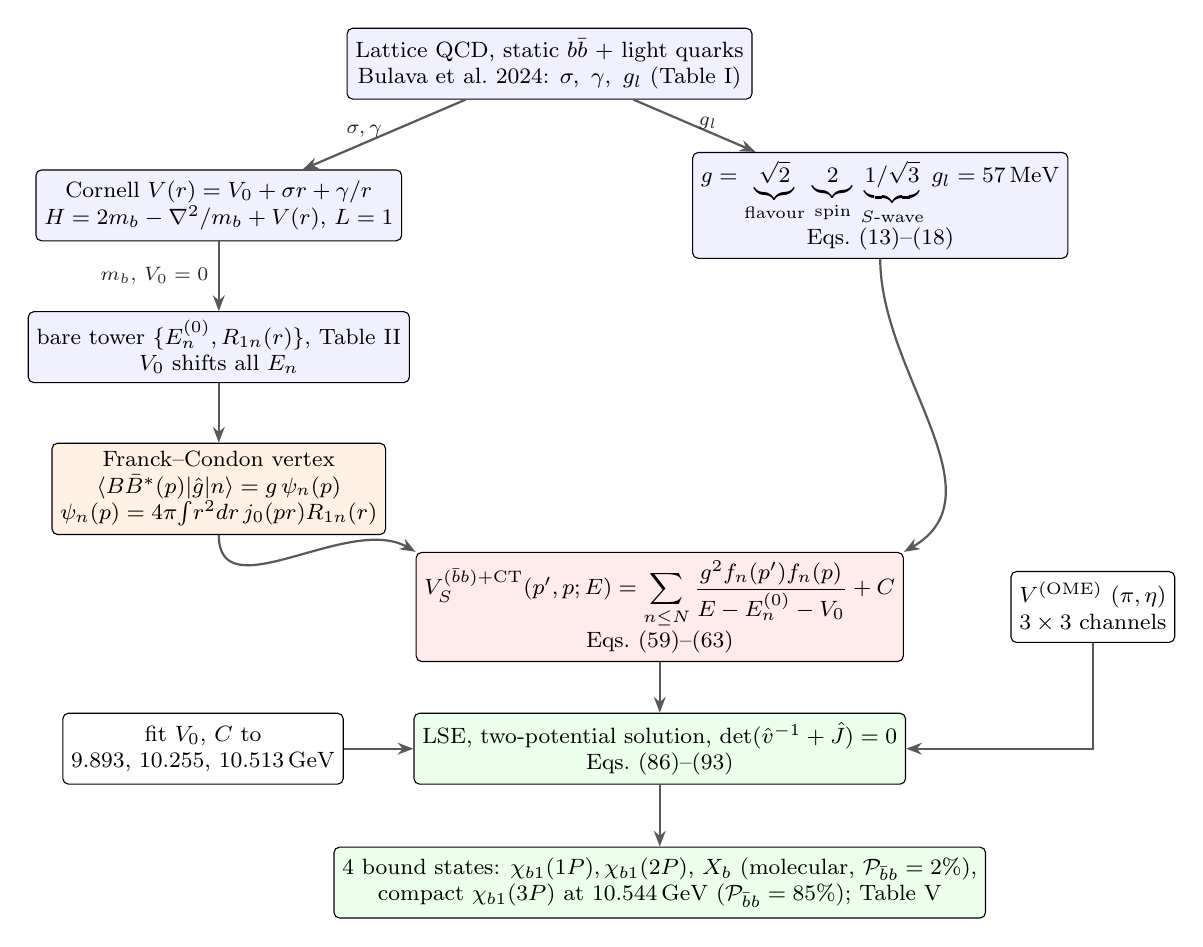
\begin{tikzpicture}[
  box/.style={draw,rounded corners=2pt,align=center,font=\footnotesize,fill=#1,inner sep=3pt,minimum height=0.9cm},
  box/.default=white,
  arr/.style={-{Stealth[length=2mm]},thick,gray!70!black},
  lab/.style={font=\scriptsize,align=center,text=gray!30!black}]
\node[box=blue!6] (lat) at (0,0) {Lattice QCD, static $b\bar b$ + light quarks\\ Bulava et al.\ 2024: $\sigma,\ \gamma,\ g_l$ (Table I)};
\node[box=blue!6] (corn) at (-4.2,-1.8) {Cornell $V(r)=V_0+\sigma r+\gamma/r$\\ $H=2m_b-\nabla^2/m_b+V(r)$, $L=1$};
\node[box=blue!6] (gch) at (4.2,-1.8) {$g=\underbrace{\sqrt2}_{\rm flavour}\,\underbrace{2}_{\rm spin}\,\underbrace{1/\sqrt3}_{S\text{-wave}}\,g_l=57\MeV$\\ Eqs.~(13)--(18)};
\node[box=blue!6] (tower) at (-4.2,-3.6) {bare tower $\{E_n^{(0)},R_{1n}(r)\}$, Table II\\ $V_0$ shifts all $E_n$};
\node[box=orange!10] (ff) at (-4.2,-5.4) {Franck--Condon vertex\\ $\langle\BBst(p)|\hat g|n\rangle=g\,\psi_n(p)$\\ $\psi_n(p)=4\pi\!\int\! r^2dr\,j_0(pr)R_{1n}(r)$};
\node[box=red!8] (V) at (1.4,-6.9) {$V_S^{(\bar bb)+{\rm CT}}(p',p;E)=\displaystyle\sum_{n\le N}\frac{g^2 f_n(p')f_n(p)}{E-E_n^{(0)}-V_0}+C$\\ Eqs.~(59)--(63)};
\node[box] (ome) at (6.9,-6.9) {$\VOME$ ($\pi,\eta$)\\ $3\times3$ channels};
\node[box=green!8] (lse) at (1.4,-8.7) {LSE, two-potential solution, $\det(\hat v^{-1}+\hat J)=0$\\ Eqs.~(86)--(93)};
\node[box] (fit) at (-4.4,-8.7) {fit $V_0$, $C$ to\\ $9.893,\,10.255,\,10.513\GeV$};
\node[box=green!8] (out) at (1.4,-10.4) {4 bound states: $\chi_{b1}(1P),\chi_{b1}(2P)$, $X_b$ (molecular, ${\cal P}_{\bar bb}=2\%$),\\ compact $\chi_{b1}(3P)$ at $10.544\GeV$ (${\cal P}_{\bar bb}=85\%$); Table V};
\draw[arr] (lat) -- node[lab,left,pos=0.45]{$\sigma,\gamma$} (corn);
\draw[arr] (lat) -- node[lab,right,pos=0.45]{$g_l$} (gch);
\draw[arr] (corn) -- node[lab,left]{$m_b$, $V_0=0$} (tower);
\draw[arr] (tower) -- (ff);
\draw[arr] (ff.south) to[out=-90,in=150] (V.north west);
\draw[arr] (gch.south) to[out=-90,in=30] (V.north east);
\draw[arr] (V) -- (lse);
\draw[arr] (ome) |- (lse);
\draw[arr] (fit) -- (lse);
\draw[arr] (lse) -- (out);
\end{tikzpicture}
\caption{The chain that produces the $s$-channel interaction and feeds it into the scattering problem. Blue: lattice/quark input; orange: the transition vertex; red: the $s$-channel potential (with the contact term attached); green: the hadronic scattering problem. Equation and table numbers refer to the paper.}
\label{fig:map}
\end{figure}

%=====================================================================
\section{Quantum numbers: a complete guide}
\label{sec:qn}
%=====================================================================

The paper uses five layers of labels. They are not independent: each layer organises the same Hilbert space so that one symmetry is manifest.
\begin{center}
\small
\begin{tabular}{>{\raggedright\arraybackslash}p{3.6cm}>{\raggedright\arraybackslash}p{4.4cm}>{\raggedright\arraybackslash}p{7.0cm}}
\toprule
layer & labels & why this basis\\
\midrule
exact symmetries & $J^{PC}$, isospin $I$ & conserved by QCD; every component of a physical state shares them\\
compact $\bar bb$ (quark model) & $n\,^{2S+1}L_J$, $[\bar bb]_1(nP)$ & eigenstates of the spin-independent Cornell Hamiltonian\\
meson pairs (partial waves) & $^{2S+1}L_J$, channel index $\alpha$ & free two-meson motion; the basis of the LSE\\
heavy-quark spin symmetry & $s_{\bar bb}^{PC}$, $j_\ell^{PC}$ & the heavy-quark spin decouples as $m_b\to\infty$\\
Born--Oppenheimer (static) & $\lambda_\ell$, $\Lambda_\eta^\sigma$, $J_\ell$ & light degrees of freedom at a fixed $b\bar b$ axis; lattice levels\\
\bottomrule
\end{tabular}
\end{center}
Sections~\ref{sec:qn-exact}--\ref{sec:qn-proj} go through the layers in this order, derive every number the paper uses, and end with a dictionary (Table~\ref{tab:qn-dict}). Results marked \tagN{} in this section were checked by explicit computation in \texttt{code/qnumbers.py}.

\subsection{Exact quantum numbers: $J^{PC}$ and isospin}
\label{sec:qn-exact}

$J$ is the total angular momentum, $P$ the parity and $C$ the charge-conjugation parity. $C$ is defined only for systems that are their own antiparticle: the $\bar bb$ states, and suitable combinations of a meson with its antimeson. The paper studies $J^{PC}=1^{++}$ \tagP{l.\,213}, the quantum numbers of $\chi_{c1}(3872)=X(3872)$ \tagP{l.\,1806--1807}, in the isoscalar sector, $I=0$, with $B$ and $B^*$ in the isospin limit \tagP{l.\,254}. The isoscalar flavour combination of a pair is $(\ket{B_u\bar B_u}+\ket{B_d\bar B_d})/\sqrt2$, where $u,d$ label the light-quark content \tagP{Eq.~(13)}.

Why these matter: QCD conserves $J$, $P$, $C$ and (in the isospin limit) $I$. A physical $1^{++}$, $I=0$ state can therefore contain only components with the same labels: the $^3P_1$ bottomonia and the meson-pair channels with $J^{PC}=1^{++}$. Everything below is about identifying these components and computing their overlaps.

\subsection{Bottomonium: $n\,^{2S+1}L_J$ and $[\bar bb]_1(nP)$}
\label{sec:qn-bb}

For a fermion--antifermion pair with orbital angular momentum $L$ and total spin $S$ (standard results; the $-1$ in $P$ is the opposite intrinsic parity of fermion and antifermion):
\begin{equation}
P=(-1)^{L+1},\qquad C=(-1)^{L+S},\qquad \bm J=\bm L+\bm S .
\end{equation}
\begin{center}
\small
\begin{tabular}{cccl}
\toprule
$L$ & $S$ & $J^{PC}$ & bottomonium\\
\midrule
0 & 0 & $0^{-+}$ & $\eta_b(nS)$\\
0 & 1 & $1^{--}$ & $\Upsilon(nS)$\\
1 & 0 & $1^{+-}$ & $h_b(nP)$\\
1 & 1 & $0^{++},\ \bm{1^{++}},\ 2^{++}$ & $\chi_{b0}(nP),\ \bm{\chi_{b1}(nP)},\ \chi_{b2}(nP)$\\
\bottomrule
\end{tabular}
\end{center}
$1^{++}$ requires $L=S=1$ and $J=1$: the $^3P_1$ states $\chi_{b1}(nP)$, or $n\,^3P_1$ in spectroscopic notation. The paper's symbol $\bbnP$ spells this out: subscript 1 for the heavy-pair spin $s_{\bar bb}=1$, $P$ for $L=1$, $n$ for the radial excitation \tagP{l.\,286--287, 738}. $R_{1n}$ has $n-1$ nodes (Fig.~\ref{fig:un}).

\paragraph{The spin multiplet.} At LO the Cornell potential is spin independent, so $\chi_{b0}$, $\chi_{b1}$, $\chi_{b2}$ with the same $n$ share $R_{1n}$ and the mass $M^{(\bar bb)}$. Spin-dependent forces split them \tagP{App.~B, Eqs.~(B1),(B2)}:
\begin{equation}
V_{\rm SD}=V_{\rm SS}(2\bm S^2-3)+V_{\rm SL}\,\bm S\cdot\bm L+V_{\rm ST}\,S_{12},\qquad S_{12}=3(\bm S\cdot\hat{\bm r})^2-\bm S^2 .
\end{equation}
For $P$ waves the wave function vanishes at the origin, so $V_{\rm SS}$ drops out. The angular factors are
\begin{center}
\small
\begin{tabular}{cccc}
\toprule
$J$ & $\braket{\bm S\cdot\bm L}=\frac12[J(J+1)-L(L+1)-S(S+1)]$ & $\braket{S_{12}}=1-\frac{9}{2J+1}\braket{1\,0\,1\,0|J\,0}^2$ & $\Delta M_{\rm SD}[\chi_{bJ}]$\\
\midrule
0 & $-2$ & $-2$ & $-2\braket{V_{\rm SL}}-2\braket{V_{\rm ST}}$\\
1 & $-1$ & $+1$ & $-\braket{V_{\rm SL}}+\braket{V_{\rm ST}}$\\
2 & $+1$ & $-\frac15$ & $\braket{V_{\rm SL}}-\frac15\braket{V_{\rm ST}}$\\
\bottomrule
\end{tabular}
\end{center}
\tagP{Eqs.~(B3),(B4)} \tagN. Both angular columns obey $\sum_J(2J+1)\braket{\cdots}=0$, so $\sum_J(2J+1)\Delta M_{\rm SD}=0$: $M^{(\bar bb)}$ is the spin-weighted centroid $\frac19\sum_J(2J+1)M[\chi_{bJ}]$ \tagP{Eqs.~(B5),(B6)}. The paper uses only $J=1$; the variation of its correction over the states used is $\approx1\MeV$ and is absorbed in $V_0$ \tagP{l.\,1998}. The paper's $S_{12}$ is half the more common $3(\bm\sigma_1\cdot\hat{\bm r})(\bm\sigma_2\cdot\hat{\bm r})-\bm\sigma_1\cdot\bm\sigma_2$, whose $^3P_J$ values are $-4,\,2,\,-\frac25$ \tagD.

\paragraph{Why these states show up in $\Upsilon\gamma$.} The E1 transition $\chi_{bJ}(nP)\to\gamma\,\Upsilon(mS)$ changes $L$ by one at fixed $S$ and conserves $C$: $(+)\to(-)(-)$ \tagD. This is the channel in which CMS measured the $3P$ states \tagP{Sect.~IV\,G}.

\subsection{Heavy--light mesons}
\label{sec:qn-B}

$B$ ($J^P=0^-$) and $B^*$ ($1^-$) contain a $b$ quark (or $\bar b$) and a light antiquark (or quark). In the heavy-quark limit the heavy-quark spin decouples from the light degrees of freedom, which carry $j^P=\frac12^-$ in the ground state. Coupling them to $s_b=\frac12$ gives $J=0$ and $J=1$, degenerate; $m_{B^*}-m_B=46\MeV$ is an ${\cal O}(1/m_b)$ effect \tagP{Eq.~(3); l.\,541: ``there is no hyperfine splitting between $B$ and $B^*$'' in the heavy-quark limit}. This is why both sit in one superfield, $H_a=P_a+\bm V_a\cdot\bm\sigma$, a $2\times2$ matrix in heavy$\otimes$light spin space, with $P_a=\{B^-,\bar B^0\}$, $V_a=\{B^{*-},\bar B^{*0}\}$ and antimesons $\bar P_a=\{B^+,B^0\}$, $\bar V_a=\{B^{*+},B^{*0}\}$ \tagP{Sect.~III\,B}. The index $a$ is the light flavour, an isospin doublet.

Charge conjugation requires a phase convention. The paper uses ${\cal C}P_a{\cal C}^{-1}=\bar P_a$, ${\cal C}V_a^i{\cal C}^{-1}=-\bar V_a^i$, ${\cal C}H_a{\cal C}^{-1}=\sigma_2\bar H_a^T\sigma_2$. With it the $C$-even pseudoscalar--vector state is \tagP{footnote 14}
\begin{equation}
\ket{B\bar B^*;C=+}=\frac{1}{\sqrt2}\big(\ket{B\bar B^*}-\ket{B^*\bar B}\big).
\end{equation}
Whenever the paper writes ``$B\bar B^*$'', it means this combination \tagP{footnote at l.\,191}.

\subsection{Meson--antimeson pairs: why exactly three channels}
\label{sec:qn-pairs}

For a pair with relative orbital angular momentum $L$ and total spin $S$ \tagD:
\begin{itemize}
\item $P=P_1P_2(-1)^L$. For $B^{(*)}\bar B^{(*)}$, $P_1P_2=(-1)(-1)=+1$, so $P=(-1)^L$: positive parity needs even $L$.
\item $C=(-1)^{L+S}$ for $B\bar B$ and $B^*\bar B^*$: charge conjugation exchanges meson and antimeson, as for $\pi^+\pi^-$ or $\rho^+\rho^-$.
\item $B\bar B^*$ alone is not a $C$ eigenstate. The combinations $(\ket{B\bar B^*}\mp\ket{B^*\bar B})/\sqrt2$ are, with $C=\pm(-1)^L$ in the paper's convention.
\end{itemize}
Enumerating all possibilities with $J=1$, $P=+$, $C=+$ \tagD:
\begin{center}
\small
\begin{tabular}{lcccl}
\toprule
pair & $S$ & $L$ & allowed $J^{PC}$ & $1^{++}$?\\
\midrule
$B\bar B$ & 0 & $L$ & $J=L$: $0^{++},1^{--},2^{++},\dots$ & no\\
$B\bar B^*$, $C$-even & 1 & 0 & $1^{++}$ & \textbf{yes: $^3S_1$, $\alpha=1$}\\
$B\bar B^*$, $C$-even & 1 & 2 & $1^{++},2^{++},3^{++}$ & \textbf{yes: $^3D_1$, $\alpha=2$}\\
$B\bar B^*$, $C$-odd & 1 & 0, 2 & $1^{+-},\dots$ & no\\
$B^*\bar B^*$ & 0 & 0 & $0^{++}$ & no\\
$B^*\bar B^*$ & 1 & 0 & $1^{+-}$ & no\\
$B^*\bar B^*$ & 2 & 0 & $2^{++}$ & no\\
$B^*\bar B^*$ & 0 & 2 & $2^{++}$ & no\\
$B^*\bar B^*$ & 1 & 2 & $1^{+-},2^{+-},3^{+-}$ & no\\
$B^*\bar B^*$ & 2 & 2 & $0^{++},\dots,4^{++}$ & \textbf{yes: $^5D_1$, $\alpha=3$}\\
any & $\le2$ & $\ge4$ & $J\ge L-S\ge2$ & no\\
\bottomrule
\end{tabular}
\end{center}
So the three channels of Eq.~(1) \emph{exhaust} the $1^{++}$ states of $B^{(*)}\bar B^{(*)}$ pairs; no partial wave was dropped by choice. Channel 3 opens $\Delta m=46\MeV$ above the other two and has reduced mass $\mu_3=m_{B^*}/2$ \tagP{Eq.~(3)}. The $1^{+-}$ rows form the sector of the (isovector) $Z_b(10610)$ and $Z_b(10650)$, which the paper mentions in its OME discussion \tagP{l.\,1073--1080}.

\subsection{Heavy-quark spin symmetry: $s_{\bar bb}\otimes j_\ell$}
\label{sec:qn-hqss}

Each meson couples a heavy-quark spin to a light spin. For a pair one can instead couple the two heavy spins to $s_{\bar bb}\in\{0,1\}$ and the two light spins to $j_\ell\in\{0,1\}$. In the heavy-quark limit $s_{\bar bb}$ is separately conserved, so this basis makes heavy-quark spin symmetry (HQSS) manifest.

\paragraph{$PC$ of the two subsystems.} The heavy-spin states carry the $PC$ of $S$-wave quarkonium with that spin, $0_{\bar bb}^{-+}$ ($\eta_b$-like) and $1_{\bar bb}^{--}$ ($\Upsilon$-like); the light-spin states likewise $0_\ell^{-+}$ and $1_\ell^{--}$ \tagP{l.\,421}. For an $S$-wave pair the $P$ and $C$ multiply and $J$ adds \tagP{Eqs.~(15),(16)}:
\begin{equation}
0_\ell^{-+}\otimes0_{\bar bb}^{-+}=0^{++},\quad
0_\ell^{-+}\otimes1_{\bar bb}^{--}=1^{+-},\quad
1_\ell^{--}\otimes0_{\bar bb}^{-+}=1^{+-},\quad
1_\ell^{--}\otimes1_{\bar bb}^{--}=0^{++}\oplus1^{++}\oplus2^{++}.
\end{equation}
\textbf{The only way to make $1^{++}$ is $j_\ell=1$ with $s_{\bar bb}=1$.}

\paragraph{The meson pairs in this basis} \tagN{} (explicit spin algebra):
\begin{center}
\small
\begin{tabular}{llc}
\toprule
$S$-wave pair & heavy $\otimes$ light decomposition & $J^{PC}$\\
\midrule
$B\bar B$ ($S=0$) & $\frac12\,0_H\otimes0_\ell+\frac{\sqrt3}{2}\,(1_H\otimes1_\ell)_0$ & $0^{++}$\\
$B^*\bar B^*$ ($S=0$) & $\frac{\sqrt3}{2}\,0_H\otimes0_\ell-\frac12\,(1_H\otimes1_\ell)_0$ & $0^{++}$\\
$B\bar B^*$, $C$-even & $(1_H\otimes1_\ell)_1$\quad (pure) & $1^{++}$\\
$B\bar B^*$, $C$-odd & $\frac{1}{\sqrt2}\big(0_H\otimes1_\ell-1_H\otimes0_\ell\big)$ & $1^{+-}$\\
$B^*\bar B^*$ ($S=1$) & $\frac{1}{\sqrt2}\big(0_H\otimes1_\ell+1_H\otimes0_\ell\big)$ & $1^{+-}$\\
$B^*\bar B^*$ ($S=2$) & $(1_H\otimes1_\ell)_2$\quad (pure) & $2^{++}$\\
\bottomrule
\end{tabular}
\end{center}
Relative signs depend on phase conventions; magnitudes do not. Exactly one of the two combinations $\ket{B\bar B^*}\pm\ket{B^*\bar B}$ is pure $(1_H\otimes1_\ell)_1$. That is the $C$-even one, as the $PC$ rule requires; in the paper's convention it carries the minus sign. The table agrees with \tagR{Bondar 2011, Eqs.~(1)--(3),(7),(8)}. The first row, written in the $m$-basis, is the paper's Eq.~(14) (Sect.~\ref{sec:g}).

Consequences for the paper:
\begin{itemize}
\item \textbf{In $S$ wave the $1^{++}$ channel is pure $s_{\bar bb}=1$, $j_\ell=1$.} The paper's ``coupling first the $\bm s_{\bar bb}$ and $\bm j_\ell$ spin states gives $S=1$ for the $C$-even $B\bar B^*$ pair and $S=2$ for $B^*\bar B^*$'' \tagP{l.\,492} is this table: in the $1^{++}$ sector the meson-pair spin $S$ coincides with the coupled $(s_{\bar bb}\otimes j_\ell)$ spin.
\item \textbf{HQSS partners.} The $j_\ell=1$ multiplet contains $1^{++}$ together with $0^{++}$ and $2^{++}$ (same $1_\ell\otimes1_H$) and $1^{+-}$ ($1_\ell\otimes0_H$) \tagP{Eq.~(16)}. For the charm analogue: ``three degenerate spin partner states with the quantum numbers $0^{++}$, $1^{+-}$, and $2^{++}$'' accompany the $1^{++}$ $X$ \tagR{Baru 2016, summary}. The paper studies only $1^{++}$; the $\chi_{b0}$ and $\chi_{b2}$ sectors are left for the future \tagP{l.\,1748}.
\item \textbf{The lattice factor 2.} The string has $s_{\bar bb}=1$ with zero projection on $\hat{\bm r}$ and vacuum light quantum numbers. It can turn only into the $\ket{1_\ell,0}\ket{1_{\bar bb},0}$ component of the pseudoscalar pair, whose amplitude is $-\frac12$ (Sect.~\ref{sec:g}).
\end{itemize}

\subsection{Born--Oppenheimer labels $\Lambda_\eta^\sigma$}
\label{sec:qn-bo}

Place the static $b$ and $\bar b$ at $\pm\bm r/2$. The light degrees of freedom see a configuration with these symmetries \tagP{l.\,469--473}:
\begin{enumerate}
\item \textbf{Rotations about $\hat{\bm r}$.} The projection $\lambda_\ell$ of $\bm j_\ell$ on $\hat{\bm r}$ is conserved. One quotes $\Lambda=|\lambda_\ell|$ and writes $\Sigma,\Pi,\Delta,\dots$ for $\Lambda=0,1,2,\dots$, as for diatomic molecules.
\item \textbf{$CP$.} Parity alone maps $\bm r/2\to-\bm r/2$: it exchanges the positions of $b$ and $\bar b$ and is not a symmetry of the configuration. Charge conjugation exchanges $b$ and $\bar b$ back, so $CP$ is. Its eigenvalue on the light degrees of freedom is $\eta=g$ ($+1$, gerade) or $u$ ($-1$, ungerade).
\item \textbf{Reflection in a plane containing $\hat{\bm r}$.} It maps $\lambda_\ell\to-\lambda_\ell$. For $\Lambda>0$ the states $\pm\lambda_\ell$ are degenerate and labelled together. For $\Lambda=0$ the state is an eigenstate with eigenvalue $\sigma=\pm$, and for light degrees of freedom of angular momentum $j_\ell$ and parity $P$ it is $\sigma=P(-1)^{j_\ell}$ \tagP{l.\,473}.
\end{enumerate}
Applying the rules (assignments as in \tagP{l.\,476--486}; the $\eta$ and $\sigma$ columns \tagD):
\begin{center}
\small
\begin{tabular}{lcccccl}
\toprule
light configuration & $j_\ell^{PC}$ & $\lambda_\ell$ & $\eta$ & $\sigma$ & label & role in the paper\\
\midrule
vacuum (string) & $0^{++}$ & 0 & $g$ & $+$ & $\Sigma_g^+$ & compact $\bar bb$, Cornell potential\\
$S$-wave pair, light triplet & $1^{--}$ & 0 & $g$ & $+$ & $\Sigma_g^{+\prime}$ & mixes with the string\\
$S$-wave pair, light triplet & $1^{--}$ & $\pm1$ & $g$ & --- & $\Pi_g$ & no direct mixing\\
$S$-wave pair, light singlet & $0^{-+}$ & 0 & $u$ & $-$ & $\Sigma_u^-$ & cannot give $1^{++}$\\
\bottomrule
\end{tabular}
\end{center}
The prime on $\Sigma_g^{+\prime}$ only distinguishes the meson-pair configuration from the string, which has identical labels. Precisely because the labels coincide, the two can mix: levels of equal symmetry cannot cross, so the string and the $\Sigma_g^{+\prime}$ pair level undergo an \emph{avoided} crossing, which is string breaking (Fig.~\ref{fig:lattice}). Configurations with other labels ($\Pi_g$, $\Sigma_u^-$) do not mix with the string in the static limit \tagR{Berwein 2024, Sect.~VI; Tarr\'us Castell\`a 2022, Eq.~(7)}. In Eq.~(14) the components $\ket{1_\ell,0}$, $\ket{0_\ell,0}$, $\ket{1_\ell,\pm1}$ are the $\Sigma_g^{+\prime}$, $\Sigma_u^-$, $\Pi_g$ pieces \tagP{l.\,486}. Why $\Sigma_u^-$ cannot give $1^{++}$ for any $L$ \tagP{l.\,505} \tagD: with $j_\ell^{PC}=0^{-+}$, $P=+$ needs even $L$; $C=+$ then needs $s_{\bar bb}=0$; then $J=L$ is even, never 1.

\subsection{From BO configurations to partial waves}
\label{sec:qn-recoupling}

$J=1$ can be built from $s_{\bar bb}=1$, $j_\ell=1$ and the relative orbital $L$ in two orders \tagP{l.\,491--495}:
\begin{itemize}
\item meson (partial-wave) basis: $\bm S=\bm j_\ell+\bm s_{\bar bb}$, then $\bm J=\bm L+\bm S$, giving the channels $^3S_1$, $^3D_1$, $^5D_1$;
\item BO basis: $\bm J_\ell=\bm L+\bm j_\ell$, then $\bm J=\bm J_\ell+\bm s_{\bar bb}$. $J_\ell$ is conserved in the heavy-quark limit because the heavy spin decouples.
\end{itemize}
\paragraph{Counting.} $L=0$ gives $J_\ell=1$. $L=2$ gives $J_\ell=1,2,3$, but $J_\ell=3$ cannot combine with $s_{\bar bb}=1$ to $J=1$. $L=1$ is excluded by parity. This leaves three states, $(L,J_\ell)=(0,1),(2,1),(2,2)$: as many as there are channels.

\paragraph{Step 1: 6$j$ recoupling at $L=2$} \tagP{Eq.~(20)}. The standard recoupling formula,
\begin{equation}
\Braket{(L\,j_\ell)J_\ell,\,s_{\bar bb};J\,\big|\,L,(j_\ell\,s_{\bar bb})S;J}=(-1)^{L+j_\ell+s_{\bar bb}+J}\sqrt{(2J_\ell+1)(2S+1)}\begin{Bmatrix}L&j_\ell&J_\ell\\ s_{\bar bb}&J&S\end{Bmatrix},
\end{equation}
with $\{2\,1\,1;1\,1\,1\}=\frac16$, $\{2\,1\,1;1\,1\,2\}=\{2\,1\,2;1\,1\,1\}=-\frac{\sqrt5}{10}$ and $\{2\,1\,2;1\,1\,2\}=-\frac1{10}$, reproduces Eq.~(20) exactly \tagN:
\begin{equation}
\ket{(2\,1)J_\ell{=}1}=-\tfrac12\ket{^3D_1}+\tfrac{\sqrt3}{2}\ket{^5D_1},\qquad
\ket{(2\,1)J_\ell{=}2}=\tfrac{\sqrt3}{2}\ket{^3D_1}+\tfrac12\ket{^5D_1}.
\end{equation}
At $L=0$ nothing needs recoupling: $\ket{(0\,1)J_\ell{=}1}=\ket{^3S_1}$. A different ordering of $j_\ell$ and $s_{\bar bb}$ inside $S$ only changes signs.

\paragraph{Step 2: from definite $L$ to definite $\lambda_\ell$} \tagP{Eq.~(21)}:
\begin{equation}
\ket{J_\ell M_\ell;\lambda_\ell}=\sum_L\sqrt{\frac{2L+1}{2J_\ell+1}}\,\braket{L\,0\,j_\ell\,\lambda_\ell|J_\ell\,\lambda_\ell}\,\ket{(L\,j_\ell)J_\ell M_\ell}.
\end{equation}
The $0$ in $\braket{L\,0\,\dots}$ expresses that the relative orbital angular momentum has no component along the axis, $\bm L\cdot\hat{\bm r}=0$ \tagP{l.\,497}. The Clebsch--Gordan coefficients needed are \tagN{} $\braket{0\,0\,1\,0|1\,0}=1$, $\braket{2\,0\,1\,0|1\,0}=-\sqrt{2/5}$, $\braket{2\,0\,1\,0|2\,0}=0$, and $\braket{L\,0\,1\,{\pm1}|1\,{\pm1}}=1,\ \mp\frac{1}{\sqrt2},\ \frac{1}{\sqrt{10}}$ for $L=0,1,2$. Hence:
\begin{itemize}
\item $\lambda_\ell=0$, $J_\ell=1$: $\ket{\Sigma_g^{+\prime}}=\frac{1}{\sqrt3}\ket{(0\,1)1}-\sqrt{\frac23}\,\ket{(2\,1)1}$;
\item $\lambda_\ell=0$, $J_\ell=2$: zero, because $\braket{2\,0\,1\,0|2\,0}=0$. This is the paper's ``the state $\ket{J_\ell=2,\lambda_\ell=0}$ does not contribute'' \tagP{l.\,497--504};
\item $\lambda_\ell=\pm1$, $J_\ell=1$: each contains an $L=1$ piece with opposite signs. The reflection-symmetric combination $(\ket{+1}+\ket{-1})/\sqrt2$ cancels it, as parity requires, leaving $\ket{\Pi_g;1}=\sqrt{\frac23}\,\ket{(0\,1)1}+\frac{1}{\sqrt3}\ket{(2\,1)1}$;
\item $J_\ell=2$: $\ket{\Pi_g;2}=\ket{(2\,1)2}$.
\end{itemize}

\paragraph{Step 3: combine.} Inserting Step 1 into Step 2 gives the orthogonal matrix Eq.~(22) of the paper (Eq.~\eqref{eq:BOmatrix} here), e.g.
\begin{equation}
\ket{\Sigma_g^{+\prime}}=\tfrac{1}{\sqrt3}\ket{^3S_1}-\sqrt{\tfrac23}\Big(-\tfrac12\ket{^3D_1}+\tfrac{\sqrt3}{2}\ket{^5D_1}\Big)=\tfrac{1}{\sqrt3}\ket{^3S_1}+\tfrac{1}{\sqrt6}\ket{^3D_1}-\tfrac{1}{\sqrt2}\ket{^5D_1}.
\end{equation}
\tagN{} $UU^T=\mathbf 1$ checked for all three rows.

\paragraph{What the matrix is used for.}
\begin{enumerate}
\item Its first row is the partial-wave content of the configuration a compact $\bbnP$ turns into. Hence the $1/\sqrt3$ in $g$ (Sect.~\ref{sec:g}).
\item It turns static BO potentials into channel matrices. With $V_{\Pi_g}$ shared by both $\Pi_g$ states \tagP{Eqs.~(25)--(27)},
\begin{gather}
V(r)=U^T{\rm diag}\big(V_{\Sigma_g^{+\prime}},V_{\Pi_g},V_{\Pi_g}\big)U=V_C\,\mathbf 1+V_T\begin{pmatrix}0&-\sqrt2&\sqrt6\\-\sqrt2&1&\sqrt3\\\sqrt6&\sqrt3&-1\end{pmatrix},\\
V_C=\tfrac13\big(V_{\Sigma_g^{+\prime}}+2V_{\Pi_g}\big),\qquad V_T=\tfrac16\big(V_{\Pi_g}-V_{\Sigma_g^{+\prime}}\big)
\end{gather}
\tagN. The tensor part $V_T$, the $\Pi_g$--$\Sigma_g^{+\prime}$ difference, is what couples $S$ and $D$ waves. Because the two static potentials coincide at short distance ($V_T=b_Tr^2+\dots$), short-range $S$--$D$ and $D$--$D$ contact terms are suppressed \tagP{Eq.~(34), l.\,668--669}.
\end{enumerate}

\paragraph{Notation in BOEFT papers.} $j_\ell\to K$; $L\to L_Q$ (Berwein) or $l_{QQ}$ (Brambilla 2026); $J_\ell\to l$; $\lambda_\ell\to\lambda$ \tagP{footnote at l.\,494} \tagR{Brambilla 2026 (2604.12603), Eq.~(4.4), ordering $[s_{QQ},(K,l_{QQ})l]J$}.

\subsection{Quantum numbers inside one-meson exchange}
\label{sec:qn-ome}

\begin{itemize}
\item $\pi$: $J^{PC}=0^{-+}$, $I=1$. $\eta$: $0^{-+}$, $I=0$. Both are pseudo-Goldstone bosons and couple derivatively, through the axial current $\bm u=-\bm\nabla\Phi/F_\pi$ \tagP{Eqs.~(65),(67)}.
\item \textbf{Parity fixes the vertices.} $B\to B\pi$ is forbidden: $0^-\to0^-0^-$ needs $L=0$ for $J=0$, giving parity $(-1)(-1)=+1\neq-1$. So there is no $BB\pi$ vertex. $B^*\to B\pi$ and $B^*\to B^*\pi$ proceed in a $P$ wave, which is why their vertices are linear in the momentum: $\propto\bm\epsilon\cdot\bm q$ and $\propto(\bm\epsilon\times\bm\epsilon'^*)\cdot\bm q$ \tagP{Eqs.~(69),(70)} \tagD.
\item \textbf{Two $P$-wave vertices give rank 0 + rank 2.} $(\bm\epsilon\cdot\bm q)(\bm q\cdot\bm\epsilon'^*)=\frac13q_iq_j[\delta_{ij}\,\bm\epsilon\cdot\bm\epsilon'^*+T_{ij}]$ \tagP{Eqs.~(78),(79)}: a central piece and a rank-2 tensor piece. The tensor changes $L$ by 2 and couples $^3S_1$ to $^3D_1$ and $^5D_1$. That is why OME connects all three channels, while the $s$-channel term feeds only $\alpha=1$ at LO.
\item \textbf{Isospin factors.} For an $I=0$ meson--antimeson pair the pion exchange carries $\bm\tau\cdot\bm\tau^c\to3$ and the $\eta$ exchange $\frac13$ \tagP{Eq.~(82), l.\,1051}. \tagD{} For two doublets in $I=0$, $\braket{\bm\tau_1\cdot\bm\tau_2}=2[I(I+1)-\frac32]=-3$; the antimeson operator is $\bm\tau^c=-\bm\tau$, which gives $+3$ (it would be $-1$ for $I=1$). The $\eta$ enters $\Phi$ as $\eta/\sqrt3$ times the unit matrix \tagP{Eq.~(67)}, giving $(1/\sqrt3)^2=\frac13$.
\item The four TOPT three-body intermediate states $\{B\bar B\phi,\,B^*\bar B^*\phi,\,B\bar B^*\phi,\,\bar B^*B\phi\}$ are labelled $\beta=1,\dots,4$ \tagP{Eq.~(71)}.
\end{itemize}

\subsection{How the projectors encode $L$, $S$ and $J$}
\label{sec:qn-proj}

The partial-wave projection of OME \tagP{Eq.~(80)} uses the Cartesian projectors of \tagP{App.~D, Eq.~(D1)}:
\begin{align}
P_i(^3S_1)&=\epsilon_i,\qquad
P_i(^3D_1)=-\tfrac{3}{\sqrt2}\,\epsilon_j\big(n_in_j-\tfrac13\delta_{ij}\big),\nonumber\\
P_i(^5D_1)&=-\tfrac{\sqrt3}{2}\,i\,\varepsilon_{ijk}\Big(\epsilon_{1j}\epsilon_{2m}+\epsilon_{1m}\epsilon_{2j}-\tfrac23\delta_{jm}\,\bm\epsilon_1\cdot\bm\epsilon_2\Big)\big(n_kn_m-\tfrac13\delta_{km}\big).
\end{align}
How to read them:
\begin{itemize}
\item the open index $i$ is the polarisation of the total $J=1$ state;
\item $\bm\epsilon$ is the $B^*$ polarisation, i.e.\ spin $S=1$;
\item the symmetric traceless combination of $\bm\epsilon_1$ and $\bm\epsilon_2$ is the spin-2 state of two vector mesons, $S=2$;
\item $n_in_j-\frac13\delta_{ij}$ with $\bm n=\hat{\bm p}$ is the rank-2 spherical tensor of $L=2$; a projector without $\bm n$ is $L=0$;
\item $\varepsilon_{ijk}$ picks the $J=1$ (vector) part of the product of the $S=2$ and $L=2$ tensors.
\end{itemize}
The normalisation $\frac{1}{2J+1}\int\frac{d\Omega}{4\pi}\,{\rm Tr}\big[P\,P^\dagger\big]=1$ \tagP{Eq.~(81)} holds for all three projectors \tagN.

\subsection{Dictionary}
\label{sec:qn-dictionary}

\noindent\begin{minipage}{\textwidth}
\centering
\small
\captionof{table}{Quantum-number labels used in the paper.}
\label{tab:qn-dict}
\setlength{\tabcolsep}{4pt}
\begin{tabular}{>{\raggedright\arraybackslash}p{2.1cm}>{\raggedright\arraybackslash}p{6.6cm}>{\raggedright\arraybackslash}p{3.6cm}>{\raggedright\arraybackslash}p{2.7cm}}
\toprule
label & meaning & values here & in the paper\\
\midrule
$J^{PC}$ & total angular momentum, parity, $C$-parity & $1^{++}$ & throughout\\
$I$ & isospin & 0 & Eqs.~(13),(82)\\
$n$ & radial quantum number of the bare state ($n-1$ nodes) & $1,\dots,N$ & Eq.~(40), Table II\\
$L$ & orbital angular momentum: $\bar bb$ relative motion, or meson--meson relative motion & 1 (compact); 0, 2, 2 (channels) & Eqs.~(1),(40)\\
$S$ & total spin: of $\bar bb$, or of the meson pair & 1 (compact); 1, 1, 2 (channels) & Eq.~(1)\\
$^{2S+1}L_J$ & spectroscopic label & $^3P_1$; $^3S_1$, $^3D_1$, $^5D_1$ & Eq.~(1)\\
$[\bar bb]_1(nP)$ & bare compact state: $s_{\bar bb}=1$, $L=1$, $n$-th radial & --- & l.\,286--287\\
$\alpha$ & channel index & 1, 2, 3 & Eq.~(1)\\
$\beta$ & TOPT three-body intermediate state & 1, \dots, 4 & Eq.~(71)\\
$s_{\bar bb}$ & total spin of $b$ and $\bar b$ & 1 & Eqs.~(14)--(16)\\
$j_\ell$ & angular momentum of the light degrees of freedom & 1 & Eqs.~(14)--(16)\\
$\lambda_\ell$ & projection of $\bm j_\ell$ on the $b\bar b$ axis & 0 ($\Sigma$), $\pm1$ ($\Pi$) & Sect.~II\,F\\
$\Lambda_\eta^\sigma$ & BO label: $\Lambda=|\lambda_\ell|$, $\eta$ = $CP$, $\sigma$ = reflection & $\Sigma_g^+$, $\Sigma_g^{+\prime}$, $\Pi_g$, $\Sigma_u^-$ & Sect.~II\,F\,1\\
$J_\ell$ & $\bm L+\bm j_\ell$ (BOEFT: $l$) & 1, 2 & Eqs.~(20)--(22)\\
$M_\ell$ & projection of $J_\ell$ on a fixed axis & --- & Eq.~(21)\\
\bottomrule
\end{tabular}
\end{minipage}

%=====================================================================
\section{Why an $s$-channel term at all?}
\label{sec:why}
%=====================================================================

\subsection{The $1^{++}$ bottomonium spectrum near the $B\bar B^*$ threshold}

In the isospin limit $m_B=5.279\GeV$, $m_{B^*}=5.325\GeV$, so $\Mth=10.604\GeV$, $\Delta m=46\MeV$, and $\mu=2.651\GeV$ \tagP{Eqs.~(2),(3)}. Three axial-vector bottomonia are established, with masses $9.893$, $10.255$ and $10.513\GeV$ \tagP{Table~II}; relative to the threshold their binding momenta $\kappa_n=\sqrt{2\mu(\Mth-M_n^{\rm exp})}$ are
\begin{equation}
\kappa_1=1.942\GeV,\qquad \kappa_2=1.360\GeV,\qquad \kappa_3=0.695\GeV \qquad\text{\tagP{Eq.~(98)}}.
\end{equation}
The third state lies only $91\MeV$ below threshold. Its binding momentum, $0.695\GeV$, is the soft scale $Q$ of the problem; it is below the chiral breakdown scale $\Lambda_\chi\approx1\GeV$ \tagP{Eq.~(7)}.

\subsection{A pure quark model is not enough}

Solving a Schr\"odinger equation with the lattice Cornell potential and fitting a single overall shift $V_0$ to the three masses gives a root-mean-square deviation of $21\MeV$ \tagP{Eq.~(42)}. The failure is structural: the theoretical difference of successive level spacings is $66\MeV$, the experimental one $104\MeV$ \tagP{Eqs.~(43),(44)}. The paper's diagnosis \tagP{l.\,777}: the quark model ``fails to reproduce the reduction of the level spacing between successive bottomonium states as the open-bottom threshold is approached, where effects from couplings to the continuum are expected to play an essential role''. Forcing the quark model to fit requires $\sigma=0.120\GeV^2$ and $\gamma=-0.920$ ($\alpha_s=0.69$) with $V_0=827\MeV$, values the paper calls unphysical \tagP{footnote at l.\,764}.

That the coupling to open-flavour channels shifts and mixes quarkonium levels is an old idea:
\begin{itemize}
\item Eichten \emph{et al.}\ (1978) built an interaction that ``describes both quark--antiquark binding and pair creation, and thereby provides a unified approach for energies below and above the threshold'' \tagR{Eichten 1978, abstract}.
\item T\"ornqvist (1985) reviews how meson loops shift hadron masses ``by up to 100's of MeV'' and generate multi-quark components \tagR{T\"ornqvist 1985, abstract}.
\item Kalashnikova (2005) set up exactly the block Hamiltonian used here (bare $c\bar c$ states + free meson pairs + transition form factors), with $Z$-factors, and found an option in which a bare $2^3P_1$ state produces a near-threshold $D\bar D^*$ virtual state whose ``admixture of the bare $c\bar c$ state \dots is very small'' \tagR{Kalashnikova 2005, Sect.~II Eqs.~(1)--(8), Conclusions}.
\end{itemize}

\subsection{Why a hadronic EFT alone cannot settle the $X_b$}

Hadronic EFTs that treat the $X_b$ as a $\BBst$ molecule depend strongly on how the short-range potential scales with the heavy-quark mass $m_Q$ \tagP{l.\,202--208}:
\begin{itemize}
\item if the contact term is $m_Q$ independent (as $t$/$u$-channel light-meson exchange is), the $X_b$ comes out much more deeply bound than the $X(3872)$;
\item $s$-channel exchanges of quarkonia ``introduce an explicit $m_Q$-dependence into the potential'' and are usually not included;
\item Cincioglu \emph{et al.}\ (2016) added such an $s$-channel bottomonium to a contact EFT and found the $X_b$ mass to depend on the coupling: at cutoff $1\GeV$ the binding drops from $65.9\MeV$ (no mixing) to $0.1\MeV$ as their mixing parameter grows \tagR{Cincioglu 2016, Table~4}. They kept only the $3P$ bottomonia and deliberately neglected the attraction from $4P$ \tagR{Cincioglu 2016, Sect.~V.3}.
\end{itemize}
\BOchiEFT\ makes the $s$-channel exchange systematic: the tower of compact states, their energies, wave functions and coupling all come from the lattice static potential; only $V_0$ and $C$ are fitted.

\subsection{What lattice QCD sees: string breaking}

For a static $b$ and $\bar b$ at distance $r$, unquenched lattice QCD shows two kinds of energy levels: the colour string, whose energy rises roughly linearly with $r$, and a pair of static--light mesons, whose energy is nearly flat. Bulava \emph{et al.}\ (2024) fit the three lowest levels with the matrix \tagR{Bulava 2024, Sect.~3 Eq.~(6)} \tagP{Eq.~(11)}
\begin{equation}
H(r)=\begin{pmatrix}V(r)&\sqrt2 g_l&g_s\\ \sqrt2 g_l&\hat E_1&0\\ g_s&0&\hat E_2\end{pmatrix},\qquad V(r)=\hat V_0+\sigma r+\frac{\gamma}{r},
\label{eq:Hfit}
\end{equation}
in the basis $\{\bar bb\text{ string},\ B\bar B,\ B_s\bar B_s\}$. Facts about this fit that matter later:
\begin{itemize}
\item all energies are measured from twice the static--light meson energy $2E_{\bar Ql}$, which cancels the static self-energy \tagR{Bulava 2024, Sect.~3 and Sect.~2 Eq.~(5)};
\item the $\sqrt2$ is a \emph{flavour} factor (two light flavours, ``a flavour factor $\sqrt{N_l}$ multiplies the mixing coefficient $g_l$''), not a spin factor \tagR{Bulava 2024, Sect.~3};
\item the mixing entries and the pair energies are constants; the earlier paper states explicitly ``we assume that the model parameters \dots are independent of the distance'' over its fit range $r/a=11$--25 \tagR{Bulava 2019, Sect.~4 after Eq.~(4.2)};
\item the string level crosses the $B\bar B$ level at $r_l^\star=1.211(7)(11)\fm$ and the $B_s\bar B_s$ level at $r_s^\star=1.336(7)(12)\fm$ \tagR{Bulava 2024, Eq.~(11)}.
\end{itemize}
Figure~\ref{fig:lattice} shows the eigenvalues of Eq.~\eqref{eq:Hfit} with the parameters of Table~\ref{tab:lattice}. The avoided crossing near $1.2\fm$ is ``string breaking''. The off-diagonal $g_l$ is the quantity the $s$-channel vertex is built from.

\begin{figure}[t]
\centering
\includegraphics[width=0.66\textwidth]{lattice_levels.pdf}
\caption{\tagN{} Eigenvalues (solid) of the lattice model Eq.~\eqref{eq:Hfit} for the physical-point parameters of Table~\ref{tab:lattice}, together with the diagonal (``diabatic'') entries (dashed). Energies relative to $2E_{\bar Ql}$. The string--$B\bar B$ crossing is at $r_l^\star=1.21\fm$ \tagR{Bulava 2024, Eq.~(11)}.}
\label{fig:lattice}
\end{figure}

\subsection{The Born--Oppenheimer selection rule}
\label{sec:BOrule}

In the static limit the $b\bar b$ axis $\hat{\bm r}$ is fixed, and light-quark/gluon states are classified by $\Lambda_\eta^\sigma$: $\Lambda=|\lambda_\ell|$ (projection of the light angular momentum $\bm j_\ell$ on $\hat{\bm r}$; $\Sigma,\Pi$ for $0,1$), $\eta=g,u$ for even/odd $PC$, and $\sigma$ (reflection, $\Lambda=0$ only) \tagP{Sect.~II\,F\,1}; definitions and derivations are in Sect.~\ref{sec:qn-bo}. Then \tagP{l.\,476--486}:
\begin{itemize}
\item the compact $\bar bb$ state (string, light degrees of freedom in the vacuum, $j_\ell^{PC}=0^{++}$) is $\Sigma_g^+$;
\item an $S$-wave meson pair with $j_\ell^{PC}=1^{--}$ splits into $\Sigma_g^{+\prime}$ ($\lambda_\ell=0$) and $\Pi_g$ ($\lambda_\ell=\pm1$); with $j_\ell^{PC}=0^{-+}$ it is $\Sigma_u^-$.
\end{itemize}
\textbf{Only $\Sigma_g^{+\prime}$ mixes directly with the compact $\Sigma_g^+$}, because the mixing must conserve the BO quantum numbers. The references agree: ``Since the quarkonium field $\Psi$ inherently belongs to a $\Lambda=0$ representation, we should project the heavy meson pair field into the same representation'' \tagR{Tarr\'us Castell\`a 2022, Sect.~II, Eq.~(7)}; the $\Pi_g$ static energy ``does not show avoided level crossing with the quarkonium'' \tagR{Berwein 2024, Sect.~VI, Eq.~(6.6)}; the mixing is renamed $V_{\Sigma_g^+\text{-}\Sigma_g^{+\prime}}$ ``to emphasize that the mixing occurs between the potentials with BO quantum numbers $\Sigma_g^+$ and $\Sigma_g^{+\prime}$'' \tagR{Brambilla 2026 (2604.12603), Eq.~(2.4)}.

For $1^{++}$ there are three BO configurations, $\{\Sigma_g^{+\prime},\Pi_g;1,\Pi_g;2\}$, related to the three partial-wave channels by an orthogonal matrix \tagP{Eq.~(22)}
\begin{equation}
\begin{pmatrix}\ket{\Sigma_g^{+\prime}}\\ \ket{\Pi_g;1}\\ \ket{\Pi_g;2}\end{pmatrix}
=\begin{pmatrix}\frac{1}{\sqrt3}&\frac{1}{\sqrt6}&-\frac{1}{\sqrt2}\\[1mm] \sqrt{\frac23}&-\frac{1}{2\sqrt3}&\frac12\\[1mm] 0&\frac{\sqrt3}{2}&\frac12\end{pmatrix}
\begin{pmatrix}\ket{\BBst(^3S_1)}\\ \ket{\BBst(^3D_1)}\\ \ket{\BstBst(^5D_1)}\end{pmatrix}.
\label{eq:BOmatrix}
\end{equation}
The first row is the partial-wave content of the configuration a compact $\bbnP$ turns into. It is the origin of the $1/\sqrt3$ in $g$ (Sect.~\ref{sec:g}). This matrix agrees with the 6$j$/9$j$ recouplings of Brambilla \emph{et al.}\ up to the overall phase of each BO state \tagR{Brambilla 2026 (2604.12603), Eqs.~(4.4),(4.6)--(4.14)}.

%=====================================================================
\section{Ingredient 1: the bare bottomonium tower}
\label{sec:tower}
%=====================================================================

\subsection{Hamiltonian and lattice parameters}

The ``bare'' states are eigenstates of \tagP{Eqs.~(37),(38)}
\begin{equation}
H\Psi^{(\bar bb)}=M^{(\bar bb)}\Psi^{(\bar bb)},\qquad H=2m_b-\frac{1}{m_b}\nabla^2+V(r),\qquad V(r)=V_0+\sigma r+\frac{\gamma}{r},
\end{equation}
with the spin-independent LO static potential in Cornell form \tagP{Eq.~(12)}. ``Bare'' means not yet coupled to the open-bottom channels \tagP{l.\,709}. The parameters come from the lattice fit, Table~\ref{tab:lattice}.

\begin{table}[h]
\centering
\caption{Lattice parameters \tagP{Table~I}, identical to Bulava 2024 Table~4 \tagR{Bulava 2024, Table~4}. Conversion with $\sqrt{t_0}=0.1443(7)(13)\fm$. Used in \BOchiEFT: $\sigma$, $\gamma$, $g_l$ (bold).}
\label{tab:lattice}
\setlength{\tabcolsep}{4pt}\small
\begin{tabular}{lccccccc}
\toprule
& $\hat E_1$ & $\hat E_2$ & $g_l$ & $g_s$ & $\sigma$ & $\hat V_0$ & $\gamma$\\
\midrule
units of $t_0$ & $0.0034(3)$ & $0.1005(7)$ & $0.0256(3)$ & $0.0134(4)$ & $0.1061(7)$ & $-0.835(7)$ & $-0.434(11)$\\
physical & $5\MeV$ & $137\MeV$ & $\bm{35\MeV}$ & $18\MeV$ & $\bm{0.198\GeV^2}$ & $-1.14\GeV$ & $\bm{-0.434}$\\
\bottomrule
\end{tabular}
\end{table}

What you should know about these numbers \tagR{Bulava 2024, Sect.~2, Table~1, Sect.~4, Eqs.~(8),(10)}:
\begin{itemize}
\item They are \emph{extrapolations to the physical quark masses} from three CLS $N_f=2+1$ ensembles with $m_\pi=340,280,200\MeV$, all at the same lattice spacing $a=0.0633\fm$ (so there is no continuum extrapolation). The extrapolation keeps $2m_l+m_s$ roughly constant.
\item Table~4 lists statistical errors only. With systematics, $g_l=35.0(5)_{\rm stat}(3)_{\rm sys}\MeV$, $g_s=18.3(6)(2)\MeV$, and $\sigma t_0=0.1061(7)(20)$, i.e.\ $\sqrt\sigma=445(3)(6)\MeV$. The paper's Table I omits the second error on $\sigma$.
\item $\gamma$ is a fitted Cornell coefficient. The paper's identification $\gamma\equiv-\frac43\alpha_s$ \tagP{Eq.~(12)} is an interpretation, not something the lattice fit imposes.
\end{itemize}
Which lattice parameters are \emph{not} used, and why \tagP{l.\,399--404}:
\begin{enumerate}[label=(\roman*)]
\item the $B_s\bar B_s^{(*)}$ channel ($\hat E_2$, $g_s$) is dropped: at the $B_s\bar B_s^*$ threshold the $\BBst$ c.m.\ momentum is $0.97\GeV\approx\Lambda_\chi$, so its effect is short-range and goes into $C$ \tagP{l.\,301};
\item $\hat V_0$ is replaced by a free $V_0$;
\item the constant pair energy $\hat E_1$ is replaced by the explicit $\BBst$ dynamics: kinetic energy, OME, and $C$.
\end{enumerate}

\subsection{$P$-wave states, the role of $m_b$ and $V_0$}

For $1^{++}$ one needs $L=s_{\bar bb}=1$, so $\Psi^{(\bar bb)}_{n,L=1}=Y_{1m}(\hat{\bm r})R_{1n}(r)$ \tagP{Eq.~(40)}. With $u_n=rR_{1n}$ the radial equation is \tagP{Eq.~(A1)}
\begin{equation}
\Big[-\frac{1}{m_b}\frac{d^2}{dr^2}+\frac{2}{m_br^2}+\sigma r+\frac{\gamma}{r}\Big]u_n(r)=\epsilon_n u_n(r),\qquad \epsilon_n=M_n^{(0)}-2m_b,\qquad \int_0^\infty dr\,u_n^2=1 .
\end{equation}
\begin{itemize}
\item \textbf{$m_b$} is needed because the lattice works at $m_b\to\infty$. The paper scans $m_b\in[4.3,5.3]\GeV$ (constituent-quark-model values up to the kinetic mass used in BOEFT) and adopts $m_b\simeq4.534\GeV$, which gives the best description of the three masses in the full calculation \tagP{Eq.~(39), l.\,729--736, Table~III}. For each $m_b$ ``the entire calculation is repeated from the beginning'' with the lattice parameters fixed.
\item \textbf{$V_0$} is first set to zero, giving the ``reference'' masses $M_n^{(0)}$ and energies $E_n^{(0)}=M_n^{(0)}-\Mth$ \tagP{l.\,745--746}. It is then restored as a free constant in the bare energies: $E_n=E_n^{(0)}+V_0$ \tagP{Eq.~(63), l.\,937--938}. $V_0$ absorbs the variation with $m_b$ and the static-to-physical difference. Spin-dependent $1/m_b^2$ corrections to the $\chi_{b1}$ masses vary by only $\approx1\MeV$ over the states used, so they are also absorbed \tagP{l.\,747, App.~B}.
\item In the quark-model calculation $V_0$ is only an overall shift. In the coupled-channel problem it is not, because the threshold $\Mth$ does not move with $V_0$: \textbf{$V_0$ sets the distances of the bare levels from the threshold}, and the $s$-channel potential depends sensitively on these distances \tagP{l.\,1230}.
\end{itemize}

The finite-difference grid uses $N_r=1.2\times10^4$ points up to $r_{\rm box}=30\GeV^{-1}\simeq5.9\fm$. The tail beyond the outer turning point is replaced by an inward Numerov solution started from the WKB logarithmic derivative at $r_{\rm far}=36\GeV^{-1}$ \tagP{App.~A, Eqs.~(A6)--(A9)}.

\begin{numbox}[Reproduction of the reference spectrum \tagN]
An independent finite-difference solution (\texttt{code/cornell.py}; $m_b=4.534048\GeV$, $\sigma=0.198406\GeV^2$, $\gamma=-0.434$, $\Mth=10.60427\GeV$) reproduces \tagP{Table~II} to the last digit:
\begin{center}
\footnotesize\setlength{\tabcolsep}{4pt}
\begin{tabular}{lccccccc}
\toprule
$n$ & 1 & 2 & 3 & 4 & 5 & 6 & 7\\
\midrule
$M_n^{(0)}$ [GeV] (this note) & 9.5232 & 9.8897 & 10.1900 & 10.4545 & 10.6956 & 10.9197 & 11.1309\\
$M_n^{(0)}$ [GeV] (paper) & 9.523 & 9.890 & 10.190 & 10.454 & 10.696 & 10.920 & 11.131\\
$E_n=E_n^{(0)}+V_0$ [MeV], $V_0=371.5\MeV$ & $-709.6$ & $-343.1$ & $-42.8$ & $221.7$ & $462.8$ & $686.9$ & $898.0$\\
rms radius [fm] & 0.41 & 0.66 & 0.87 & 1.05 & 1.22 & 1.38 & 1.53\\
$f_n(0)$ [GeV$^{-3/2}$] & 14.40 & 19.56 & 24.85 & 28.28 & 32.11 & 34.88 & 38.02\\
\bottomrule
\end{tabular}
\end{center}
The quark-model-only shift comes out $V_0^{(\bar bb)}=352.9\MeV$ with $\Delta M=20.9\MeV$, and the level-spacing differences $66.2\MeV$ (theory) vs $104.7\MeV$ (experiment), matching \tagP{Eqs.~(42)--(44)}. The row $E_n^{(0)}+V_0$ uses the \emph{full-fit} $V_0=371.5\MeV$ (\texttt{HadronDynamics.jl/data/bochiEFT/central.toml}; Table III rounds to 371). These are the bare energies that actually enter the final calculation; Table~II of the paper lists them for the quark-model-only $V_0=353\MeV$.
\end{numbox}

\begin{figure}[t]
\centering
\includegraphics[width=0.62\textwidth]{un_r.pdf}
\caption{\tagN{} Reduced radial wave functions $u_n(r)=rR_{1n}(r)$ of the bare $P$-wave tower ($n\le4$ solid, $5\le n\le7$ dashed). The dotted line marks where the lattice string level crosses the $B\bar B$ level ($r_l^\star\approx1.2\fm$). The $n=3$ state, the one closest to threshold after the $V_0$ shift, has its outer lobe near this distance.}
\label{fig:un}
\end{figure}

%=====================================================================
\section{Ingredient 2: the coupled-channel Hamiltonian}
\label{sec:hamiltonian}
%=====================================================================

At this stage the paper isolates the $S$-wave $\BBst$ component, the only one the compact states couple to at LO; the $D$ waves come back in the full partial-wave equation through OME \tagP{l.\,784}.

\subsection{State vector and Hamiltonian}

The physical state is a superposition of the whole compact tower and the $S$-wave continuum \tagP{Eqs.~(45),(46)}:
\begin{equation}
\ket{\Psi}=\begin{pmatrix}\lambda_1\ket{\bbar_1(1P)}\\ \lambda_2\ket{\bbar_1(2P)}\\ \vdots\\ \phi(q)\ket{\BBst}\end{pmatrix},\qquad
\sum_n|\lambda_n|^2+\int\frac{q^2dq}{(2\pi)^3}|\phi(q)|^2=1 .
\label{eq:state}
\end{equation}
The spin--angular wave function of the pair is inside the ket $\ket{\BBst}$. It satisfies $\mathcal H\ket{\Psi(E)}=E\ket{\Psi(E)}$ with \tagP{Eqs.~(47),(48)}
\begin{equation}
\mathcal H=\begin{pmatrix}
H-\Mth&0&\cdots&\hat g\\
0&H-\Mth&\cdots&\hat g\\
\vdots&\vdots&\ddots&\vdots\\
\hat g&\hat g&\cdots&H_{\rm MM}
\end{pmatrix}.
\label{eq:H}
\end{equation}
Read the structure:
\begin{itemize}
\item the compact block is diagonal: bare states do not talk to each other directly;
\item every bare state couples to the \emph{same} continuum through the same transition operator $\hat g$;
\item $H_{\rm MM}$ is the meson--meson Hamiltonian (kinetic energy plus the hadron--hadron interaction).
\end{itemize}
The same block structure, for one or several bare states and one or several channels, is used in Baru \emph{et al.}\ (2010), Hanhart \emph{et al.}\ (2011), Kalashnikova (2005) and Hanhart--Nefediev (2022) \tagR{Baru 2010, Eqs.~(1)--(7); Hanhart 2011, Eqs.~(5)--(8); Kalashnikova 2005, Eqs.~(1)--(4); Hanhart 2022, Eqs.~(1)--(5)}.

\subsection{Component equations}

\begin{derbox}[Component equations \tagD]
Write $\ket{\Psi}=\sum_m\lambda_m\ket{m}+\int\frac{q^2dq}{(2\pi)^3}\phi(q)\ket{\BBst(q)}$ with $\ket{m}\equiv\ket{\bbar_1(mP)}$ and $(H-\Mth)\ket{m}=E_m\ket{m}$. Project $\mathcal H\ket\Psi=E\ket\Psi$ onto $\bra{n}$ and onto the meson sector:
\begin{align}
\lambda_nE_n+\int\frac{q^2dq}{(2\pi)^3}\phi(q)\braket{n|\hat g|\BBst(q)}&=\lambda_nE,\label{eq:sys1}\\
\sum_n\lambda_n\hat g\ket{n}+H_{\rm MM}\ket{\BBst}&=E\ket{\BBst}.\label{eq:sys2}
\end{align}
This is \tagP{Eq.~(49)}. Only the matrix element $\braket{n|\hat g|\BBst}$, the transition form factor, is left to specify.
\end{derbox}

Two equivalent routes lead from here:
\begin{enumerate}
\item eliminate the compact components $\lambda_n$, which gives an energy-dependent $\BBst$ potential. This is the paper's route (Sect.~\ref{sec:potential});
\item eliminate the continuum, which gives a self-energy $\Sigma(E)$ for the bare states and the pole equation $E-E_0-\Sigma(E)=0$. This is the route of Kalashnikova \tagR{Kalashnikova 2005, Eqs.~(5),(6)} and of the reduced matrix in Eq.~(93) of the paper (Sect.~\ref{sec:lse}).
\end{enumerate}
The \texttt{HadronDynamics.jl} implementation has both: a reduced matrix of compact states plus contact (\texttt{compact\_matrix}) and an augmented matrix that keeps the compact tower explicitly and is used to validate roots (\texttt{augmented\_matrix}) \tagR{HadronDynamics.jl, \texttt{docs/BOCHIEFT.md}, ``Bound poles and normalization''}.

%=====================================================================
\section{Ingredient 3: the transition vertex}
\label{sec:vertex}
%=====================================================================

\subsection{Coordinate-space wave functions}

The free $S$-wave pair and the bottomonium are, in coordinate space \tagP{Eqs.~(50),(51)},
\begin{equation}
\braket{\bm r|\BBst}=4\pi j_0(pr)\,\calY^{J=1}_{L=0,S=1}(\BBst;\hat{\bm r}),\qquad
\braket{\bm r|\bbnP}=R_{1n}(r)\,\calY^{J=1}_{L=1,S=1}(\bar bb;\hat{\bm r}).
\end{equation}
Here $\calY$ are spin--angular functions with total spin $J=1$, normalised so that $\int d\Omega|\calY|^2=1/(4\pi)$: a factor $1/\sqrt{4\pi}$ is put into the angular part \tagP{footnote to Eq.~(31)}. Keep this in mind; it is where the $1/(4\pi)$ in the potential comes from.

\subsection{Franck--Condon: the heavy quarks are spectators}

Fig.~\ref{fig:transition} (the paper's Fig.~1) is the picture: the $b$ and $\bar b$ go straight through, and the transition operator $\hat g$ creates a light $q\bar q$ pair.

\begin{figure}[h]
\centering
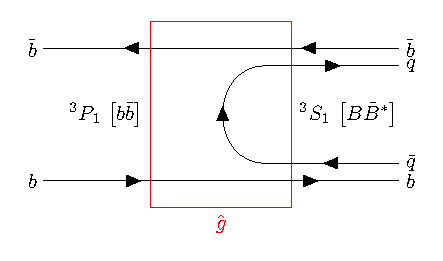
\includegraphics[width=0.42\textwidth]{diagram.pdf}
\caption{The paper's Fig.~1: the $^3P_1$ bottomonium turns into an $S$-wave $\BBst$ pair through $\hat g$; the heavy quark lines are spectators.}
\label{fig:transition}
\end{figure}

The physical assumption: the light degrees of freedom rearrange fast compared with the heavy-quark motion, so the $b\bar b$ separation $r$ is the same before and after the transition \tagP{l.\,858--861}. The coordinate $r$ is the $b\bar b$ separation in the compact channel and the meson--meson separation in the open channel; ``these two definitions agree at LO in the heavy mass expansion, since the heavy-quark positions are preserved during the transition''. The paper calls Eq.~\eqref{eq:FC} below ``a particular implementation of the Franck--Condon principle''.

What the cited Franck--Condon papers support, and what they do not:
\begin{itemize}
\item In molecules there is ``no appreciable change in the internuclear coordinate separation or momentum'' during the electronic transition. Applied to heavy hadrons: ``the heavy-quark momentum distribution in the decaying hadron coincides with the momentum distribution of the decay-product hadrons each carrying a heavy quark'', up to ${\cal O}(\Lambda_{\rm QCD}/M_Q)$ \tagR{Llanes-Estrada 2008, p.~1}. The final $B$ velocity distribution equals the initial $b$ velocity distribution up to $\Lambda_{\rm QCD}/m_b$ corrections \tagR{Torres-Rincon 2010, p.~2 below Eq.~(3)}.
\item These papers support the \emph{spectator} idea. They do not derive the specific overlap formula below or an $n$-independent $g$; those are the paper's LO assumptions (local, $r$-independent $\hat g$).
\end{itemize}

\subsection{The vertex function}

\begin{derbox}[Derivation of the vertex \tagD]
Take $\hat g$ local in $\bm r$ (Franck--Condon) and, at LO, $r$-independent, so that it acts only on the spin--angular variables. Then
\begin{align}
\braket{\BBst(p)|\hat g|\bbnP}
&=\int d^3r\;\big[4\pi j_0(pr)\calY_{0,1}^*\big]\;\hat g\;\big[R_{1n}(r)\calY_{1,1}\big]\nonumber\\
&=\underbrace{4\pi\!\int_0^\infty\! r^2dr\,j_0(pr)R_{1n}(r)}_{\psi_n(p)}\;\times\;\underbrace{\int d\Omega\,\calY^{*}_{0,1}(\BBst;\hat{\bm r})\,\hat g\,\calY_{1,1}(\bar bb;\hat{\bm r})}_{g}
=g\,\psi_n(p),
\label{eq:FC}
\end{align}
which is \tagP{Eqs.~(52)--(54)}. The constant $g$ collects the whole spin/angular recoupling between the $^3P_1$ $\bar bb$ state and the $^3S_1$ meson pair. It is $n$-independent by construction.
\end{derbox}

\begin{keybox}[Why $j_0$ and not $j_1$? The single most important conceptual point]
$\psi_n(p)$ is \textbf{not} the momentum-space wave function of the $P$-wave bottomonium, which would be a $j_1$ transform. The compact state stays a $P$ wave; the $j_0$ belongs to the free $S$-wave meson pair it overlaps with. The angular momentum $L=1$ of the $b\bar b$ relative motion is \emph{transferred to the light-quark spin}: the created light pair is in the $\Sigma_g^{+\prime}$ configuration, $j_\ell=1$ polarised along $\hat{\bm r}$. Combining the two factors of $\hat{\bm r}$ leaves an isotropic (L=0) piece with the \emph{same radial function} (box below). The \texttt{HadronDynamics.jl} documentation puts it in one line: ``The $j_0$ belongs to the continuum transition operator; the compact state remains a $P$ wave'' \tagR{HadronDynamics.jl, \texttt{docs/BOCHIEFT.md}}.

Historical note: the project's working log records that the form factor was first taken as the $j_1$ transform and later ``updated \dots to be Fourier transform of the radial wavefunction'' (\texttt{old/discussion-old.tex}, update of 15.07.2026). Expect this question from the audience.
\end{keybox}

\begin{derbox}[Where the $S$ wave comes from: a Cartesian check of the $1/\sqrt3$ \tagD]
For a $^3P_1$ state with polarisation $\bm e$, the spin--angle structure is the $J=1$ (cross-product) coupling of the orbital vector $\hat{\bm r}$ and the heavy-spin vector $\bm S$: $\propto\bm e\cdot(\hat{\bm r}\times\bm S)$. Two facts fix the transition. Heavy-quark spin symmetry keeps $\bm S$ unchanged \tagR{Bruschini 2023, Sect.~3: ``HQSS implies that the $Q$ and $\bar Q$ spins are conserved''}. The created light pair is in $\Sigma_g^{+\prime}$: light spin $j_\ell=1$ with projection $\lambda_\ell=0$ on $\hat{\bm r}$, i.e.\ a light-spin vector $\bm\ell$ entering as $\hat{\bm r}\cdot\bm\ell$. So the pair is created in
\begin{equation}
\bm e\cdot(\hat{\bm r}\times\bm S)\,(\hat{\bm r}\cdot\bm\ell)=\epsilon_{ijk}e_iS_k\ell_m\,\hat r_j\hat r_m,\qquad
\hat r_j\hat r_m=\tfrac13\delta_{jm}+\big(\hat r_j\hat r_m-\tfrac13\delta_{jm}\big).
\end{equation}
The isotropic piece is the $L=0$ part, $\frac13\,\bm e\cdot(\bm\ell\times\bm S)$: heavy and light spins coupled to total spin 1, which for $1^{++}$ is $\BBst(^3S_1)$. The traceless piece is $L=2$. Probability of the $L=0$ part: with $A_{ikm}=\epsilon_{ijk}\hat r_j\hat r_m$, $\sum_{ikm}\langle|A_{ikm}|^2\rangle_\Omega=\sum_{ijk}\epsilon_{ijk}^2/3=2$, while $\sum_{ikm}|\epsilon_{imk}/3|^2=6/9=2/3$. The $S$-wave fraction is $(2/3)/2=1/3$, i.e.\ amplitude $1/\sqrt3$, the first entry of Eq.~\eqref{eq:BOmatrix}. The radial function is untouched throughout, hence $j_0(pr)R_{1n}(r)$.
\end{derbox}

\subsection{Properties of $f_n(p)=\psi_n(p)/\sqrt{4\pi}$}

The paper works with $f_n(p)=\psi_n(p)/\sqrt{4\pi}=\frac{\sqrt{4\pi}}{p}\int_0^\infty dr\,u_n(r)\sin(pr)$, with the phase fixed by $f_n(0)>0$ \tagP{Eqs.~(61),(A10)}.
\begin{itemize}
\item \textbf{Normalisation and orthogonality} \tagD: the $j_0$ (Hankel) transform is unitary,
\begin{equation*}
\int_0^\infty p^2dp\,\Big|\sqrt{\tfrac{2}{\pi}}\int_0^\infty r^2dr\,j_0(pr)R(r)\Big|^2=\int_0^\infty r^2dr\,|R(r)|^2 .
\end{equation*}
Hence
\begin{equation}
\int_0^\infty\frac{p^2dp}{2\pi^2}\,f_n(p)f_m(p)=\delta_{nm}.
\end{equation}
\tagN{} Numerically $1.0000$ for $n=1,\dots,7$. The \texttt{HadronDynamics.jl} README states the same normalisation.
\item \textbf{Shape} (Fig.~\ref{fig:fn}) \tagN: $f_n(0)=\sqrt{4\pi}\int dr\,r\,u_n(r)$ \emph{grows} with $n$ (14.4 to 38.0 GeV$^{-3/2}$ for $n=1$--7) because the excited states are larger. Higher states are concentrated at small $p$ and have nodes: $f_3$ and $f_4$ change sign below $0.5\GeV$. The higher states are therefore \emph{not} suppressed at small momentum by the form factor; what suppresses them near threshold is the energy denominator (Sect.~\ref{sec:counting}).
\item \textbf{Imaginary momentum} \tagP{Eq.~(A11)}: the on-shell sub-threshold amplitude needs
\begin{equation*}
f_n(i\kappa)=\frac{\sqrt{4\pi}}{\kappa}\int_0^\infty dr\,u_n(r)\sinh(\kappa r).
\end{equation*}
It converges because the confined wave function falls like $\exp(-\frac23\sqrt{m_b\sigma r^3})$, faster than any exponential. This is why the tail of $u_n$ is computed carefully. For bound states \emph{on} the physical sheet the loop momenta are real, so only real-$p$ values are needed in the loops.
\item \textbf{Complex momenta}: away from the real axis use the bilinear form $\psi_n(p')\psi_n^*(p^*)$, the analytic continuation \tagP{footnote to Eq.~(58)}.
\end{itemize}

\begin{figure}[t]
\centering
\includegraphics[width=0.62\textwidth]{fn_p.pdf}
\caption{\tagN{} Vertex functions $f_n(p)$ for the bare tower at $m_b=4.534\GeV$. The dotted line marks the $X_b$ binding momentum $\kappa=0.695\GeV$, the typical loop-momentum scale of the near-threshold states.}
\label{fig:fn}
\end{figure}

%=====================================================================
\section{Ingredient 4: the coupling $g$ from lattice QCD}
\label{sec:g}
%=====================================================================

The paper converts the lattice off-diagonal entry $\sqrt2g_l$ of Eq.~\eqref{eq:Hfit} into the coupling $g$ of a $1^{++}$ bottomonium to an $S$-wave $\BBst$ pair in three steps \tagP{l.\,406--452}.

\subsection{Step 1: flavour, $\sqrt2$}
The lattice $B\bar B$ state is the normalised isoscalar $\ket{B\bar B}=(\ket{B_u\bar B_u}+\ket{B_d\bar B_d})/\sqrt2$ \tagP{Eq.~(13)}, so its mixing with the string is $\sqrt2g_l=49.5\MeV$.

\subsection{Step 2: spin overlap, factor 2}

The lattice two-meson operator is a product of two \emph{pseudoscalar} static--light mesons, $(\bar Q\gamma_5q)(\bar q\gamma_4\gamma_5Q)$ \tagR{Bulava 2019, Sect.~2.1, Eq.~(2.2)}, and $B_i=\bar Q\gamma_5q^i$ in Bali \emph{et al.}\ \tagR{Bali 2005, Sect.~II.B}. The string operator couples the heavy spins symmetrically, ``which has a zero component of angular momentum projected along $\bm r$'' \tagR{Bulava 2019, Sect.~2.1}, i.e.\ $\ket{1_{\bar bb},0}$ \tagP{l.\,433}.

\begin{derbox}[Spin decomposition of a pseudoscalar pair, Eq.~(14) \tagD]
Each meson is a heavy--light spin singlet, $(\ket{\uparrow_b\downarrow_\ell}-\ket{\downarrow_b\uparrow_\ell})/\sqrt2$, and the same for the antimeson. Multiply and regroup into heavy ($b\bar b$) and light ($\ell\bar\ell$) pairs:
\begin{equation*}
\tfrac12\Big[\ket{\uparrow\uparrow}_H\ket{\downarrow\downarrow}_L-\ket{\uparrow\downarrow}_H\ket{\downarrow\uparrow}_L-\ket{\downarrow\uparrow}_H\ket{\uparrow\downarrow}_L+\ket{\downarrow\downarrow}_H\ket{\uparrow\uparrow}_L\Big].
\end{equation*}
With $\ket{\uparrow\downarrow}=(\ket{1,0}+\ket{0,0})/\sqrt2$ and $\ket{\downarrow\uparrow}=(\ket{1,0}-\ket{0,0})/\sqrt2$ the two middle terms become $-\ket{1,0}_H\ket{1,0}_L+\ket{0,0}_H\ket{0,0}_L$. Hence
\begin{equation}
\ket{B\bar B}=\tfrac12\ket{0_\ell,0}\ket{0_{\bar bb},0}+\tfrac12\big[\ket{1_\ell,{+}1}\ket{1_{\bar bb},{-}1}+\ket{1_\ell,{-}1}\ket{1_{\bar bb},{+}1}-\ket{1_\ell,0}\ket{1_{\bar bb},0}\big],
\end{equation}
which is \tagP{Eq.~(14)}, $(-1)^{\lambda_\ell+1}/2$. Equivalently $\ket{B\bar B}=\frac12\ket{0_H0_L}+\frac{\sqrt3}{2}\ket{(1_H1_L)_0}$ \tagR{Bondar 2011, Eq.~(8)}. Bruschini writes the same source as an operator identity with different field-ordering phases; the coefficient of the longitudinal ($\Sigma$) component is $-1/2$ in both \tagR{Bruschini 2023, Eqs.~(3.1a),(3.3a)}.
\end{derbox}

Since heavy spins are conserved, the string couples only to the component with $\ket{1_{\bar bb},0}$ and light state $\ket{1_\ell,0}$, which is the $\Sigma_g^{+\prime}$ component, with coefficient $-1/2$. Bruschini: $G^{g,0}_{Q\bar Q(1),B\bar B(0)}(r)=-g(r)/2$ \tagR{Bruschini 2023, Eq.~(3.3a)}; Bicudo \emph{et al.}\ decompose Bali's operator into four BO sectors with the $\Sigma_g^+$ part carrying $-\frac12$ \tagR{Bicudo 2019, Sect.~III, Eq.~(90)}. So
\begin{equation}
\text{measured}\ \sqrt2g_l=\big|{-\tfrac12}\big|\,g_\Sigma\quad\Longrightarrow\quad g_\Sigma=2\sqrt2g_l\approx99\MeV
\end{equation}
is the mixing of the string with the \emph{normalised} $\Sigma_g^{+\prime}$ pair configuration \tagP{l.\,434} \tagD.

\begin{warnbox}[The factor 2 is an approximation; know its history]
\begin{itemize}
\item Bali \emph{et al.}\ (2005) define the mixing through a normalised two-state analysis and find, at the string-breaking point, $g(r_c)\approx\Delta E_c/2\approx25(2)\MeV$, with $r_c\approx1.25\fm$, $m_\pi\approx654\MeV$ ($am_\pi=0.276$, $a^{-1}\approx2.37\GeV$) \tagR{Bali 2005, Sect.~V.B--C, Eqs.~(90)--(95), Table~I}.
\item Bicudo \emph{et al.}\ (2019) refit a parametrisation of Bali's correlators, allowing for the four sectors. Near $r/a=15.008$ the mixing goes from $ag=0.0110(5)$ ($\approx26\MeV$) to $aV_{\rm mix}=-0.021(4)$ ($\approx50\MeV$), a ratio $\approx1.9$ \tagR{Bicudo 2019, Table~IV vs Bali 2005, Table~I}. The refit also changes the energies and the mixing angle, so it is not a pure rescaling, and it rests on extra assumptions (equal overlaps, $V_0^{\Sigma_u^-}=V_0^{\Pi_g}=0$).
\item No such reanalysis exists for the Bulava 2024 data. The paper applies the factor 2 ``pending a reanalysis'' and calls it ``a sound approximation'' \tagP{l.\,456}.
\item Earlier drafts used $g=\sqrt2g_l=49.5\MeV$ (\texttt{old/Xb-20260824.tex}, Eq.~(g)). \texttt{HadronDynamics.jl} keeps this as \texttt{coupling\_convention=:original}; the paper uses \texttt{:corrected} $=\frac{2}{\sqrt3}\sqrt2g_l$, and switching ``requires recalibration'' \tagR{HadronDynamics.jl, \texttt{docs/BOCHIEFT.md}}.
\end{itemize}
\end{warnbox}

\subsection{HQSS multiplets: which $J^{PC}$ the $\Sigma$ component feeds}
For $S$-wave pairs, the $j_\ell=0$ multiplet contains $0^{++}$ and $1^{+-}$, and the $j_\ell=1$ multiplet contains $1^{+-}$ and $0^{++}\oplus1^{++}\oplus2^{++}$ \tagP{Eqs.~(15),(16)}. The $1^{++}$ system comes from $1_\ell^{--}\otimes1_{\bar bb}^{--}$ \tagP{l.\,432}. This is consistent with Bondar \emph{et al.}\ and with the HQSS-partner counting of Baru \emph{et al.}\ \tagR{Bondar 2011, Eqs.~(1)--(8); Baru 2016, Eq.~(16)}. The full derivation, with every pair decomposed into heavy $\otimes$ light spin, is in Sect.~\ref{sec:qn-hqss}.

\subsection{Step 3: the $S$-wave share, $1/\sqrt3$}

The normalised $\Sigma_g^{+\prime}$ configuration distributes over the partial waves as the first row of Eq.~\eqref{eq:BOmatrix} \tagP{Eq.~(17)}:
\begin{equation}
\ket{\bbnP}\to\tfrac{1}{\sqrt3}\ket{\BBst(^3S_1)}+\tfrac{1}{\sqrt6}\ket{\BBst(^3D_1)}-\tfrac{1}{\sqrt2}\ket{\BstBst(^5D_1)},\qquad\tfrac13+\tfrac16+\tfrac12=1 .
\end{equation}
Bruschini's Table 2 has the same magnitudes, with a \emph{positive} $^5D_1$ coefficient: a basis-phase convention, as the paper's footnote says. The caption states the sum rule: ``for each $J^{PC}$ and each $l$ within it, the sum of the squares of the coefficients over $l'$ and the 4 di-meson channels is 1'' \tagR{Bruschini 2023, App.~D, Table~2}.

\subsection{Result}

\begin{keybox}[The coupling, Eq.~(18) of the paper]
\begin{equation}
g=\underbrace{\sqrt2}_{\text{flavour}}\times\underbrace{2}_{\text{spin overlap}}\times\underbrace{\tfrac{1}{\sqrt3}}_{S\text{-wave share}}\times g_l=\frac{2}{\sqrt3}\sqrt2\,g_l=57\MeV\quad(57.15\MeV\ \text{for}\ g_l=35.0\MeV).
\end{equation}
The three factors are distinct and must not be interchanged. The $\sqrt2$ belongs to the lattice parametrisation, the 2 corrects the pseudoscalar-operator overlap, and $1/\sqrt3$ is the $S$-wave projection of $\Sigma_g^{+\prime}$.
\end{keybox}

\subsection{What is \emph{assumed} about $g$}
\label{sec:gassump}

\paragraph{Only the $S$ wave couples at LO.} The BO selection rule picks $\Sigma_g^{+\prime}$, but $\Sigma_g^{+\prime}$ is \emph{not} a pure $S$ wave: the $D$-wave amplitudes $1/\sqrt6$ and $-1/\sqrt2$ are of the same static/HQSS order \tagR{Bruschini 2023, Table~2}. Dropping them at LO is a separate low-momentum argument: in the Franck--Condon overlap a $D$-wave vertex would involve $j_2(pr)={\cal O}((pr)^2)$ instead of $j_0(pr)=1+{\cal O}((pr)^2)$ \tagR{Tarr\'us Castell\`a 2022, Eq.~(16): the partial-wave vertex is a radial integral of $r^2\phi_{nl}V_{\rm mix}j_{l'}(kr)$}. The paper: at higher orders ``also the coupling of the $\bar bb$ states to the $D$-wave two-hadron states needs to be included, thus turning $\VQQ$ to a matrix in the channel space'' \tagP{l.\,893}. Phrase it this way in the talk. HQSS or cylindrical symmetry alone does \emph{not} remove the $D$ waves.

\paragraph{$g$ is $r$-independent and $n$-independent.} This follows the lattice parametrisation (constant mixing over the fit range). The paper adds that the $r$-dependence studied in pNRQCD ``translates to a $Q^2$-dependence that is of subleading order'' \tagP{l.\,458--461}. What the literature says about $r$-dependence:
\begin{itemize}
\item Bali extracts an $r$-dependent $g(r)$: about $320\MeV$ near $0.2\fm$, decreasing to about $25\MeV$ in the breaking region; he attributes the medium-range maximum to meson exchange \tagR{Bali 2005, Sect.~V.C Fig.~18, Sect.~VI.B}.
\item Bicudo \emph{et al.}\ use $V_{\rm mix}(r)=\sum_j c_{{\rm mix},j}\,r\,e^{-r^2/(2\lambda_{{\rm mix},j}^2)}$ \tagR{Bicudo 2019, Eqs.~(95)--(97)}.
\item In pNRQCD the mixing vanishes linearly at short distance; Tarr\'us Castell\`a uses $c_1r+c_2r^3$ (short) and $c_3/r^3$ (long) \tagR{Tarr\'us Castell\`a 2022, Eqs.~(67)--(73)}; Brambilla \emph{et al.}\ use $g\,r/r_1$ for $r<r_1=0.95\fm$, $g$ up to $r_2=1.51\fm$, then $g\,e^{-(r-r_2)/r_0}$ with $r_0=0.5\fm$ and $g=0.05\GeV$ fitted to Bulava 2024 (ensemble D200) \tagR{Brambilla 2026 (2604.12603), Eq.~(2.9), Sect.~II\,C, Fig.~1}.
\end{itemize}
\begin{numbox}[How much would an $r$-dependent mixing change the vertices? \tagN]
Replace $g\to g\,w(r)$ inside the overlap, with $w(r)$ the shape of Brambilla \emph{et al.}'s Eq.~(2.9) normalised to 1 on the plateau, and compare with constant $g$ (\texttt{code/rdep.py}):
\begin{center}
\small
\begin{tabular}{lccccccc}
\toprule
$n$ & 1 & 2 & 3 & 4 & 5 & 6 & 7\\
\midrule
$f_n^{w}(0)/f_n(0)$ & 0.55 & 0.91 & 1.00 & 0.96 & 0.77 & 0.54 & 0.29\\
$f_n^{w}(0.3\GeV)/f_n(0.3\GeV)$ & 0.53 & 0.91 & 1.02 & 1.01 & 0.81 & 0.65 & (node)\\
\bottomrule
\end{tabular}
\end{center}
For this one profile, the near-threshold $n=3$ (and $n=4$) vertex is unchanged to a few per cent, while the $n=1$ vertex is halved. The normalisation change is ${\cal O}(1)$, not ${\cal O}(Q^2)$, for the deep and the highly excited states. This is a diagnostic of one model profile, not a claim of the paper. If asked: the claim at l.\,459 is the paper's power-counting statement, and the cited BOEFT references do not establish it by themselves (they show $r$-dependent mixing; turning it into momentum-independent threshold vertices needs a matching step) \tagR{Tarr\'us Castell\`a 2022, Sect.~V; spin-recoupling audit}.
\end{numbox}

\paragraph{Lattice input without explicit meson exchange.} The Bulava fit matrices contain no pion-exchange term (``a noninteracting pair'', constant asymptotic pair levels) \tagR{Bulava 2019, Sect.~4; Bulava 2024, Eq.~(6)}. The paper argues that the avoided crossing occurs beyond $1/m_\pi$ of the lattice ensembles, so $g_l$ is a reasonable approximation, and leaves the impact of OME on these parameters for further study \tagP{l.\,726}. Bali notes meson-exchange features in his data \tagR{Bali 2005, Sect.~VI.B}.

\paragraph{Light-quark-mass dependence.} The mixing depends strongly on the light-quark mass. At the physical point $g_l/g_s\simeq1.91$ and $\sqrt2g_l\simeq49.5\MeV$ \tagR{Bulava 2024, Sect.~4, Fig.~6}.

\begin{warnbox}[Citation slip in the paper, l.\,455]
The paper attributes the ``chirally extrapolated result, $\sqrt2g_l\approx50\MeV$'' and the pion-mass dependence ``(see Fig.~6 therein)'' to Ref.~[Bulava:2019iut]. Both are in \textbf{Bulava 2024} [Bulava:2024jpj] (Sect.~4, Eq.~(8), Fig.~6). Bulava 2019 uses a single ensemble ($m_\pi=280\MeV$), has only three figures, quotes $g_1=47.2(1.4)\MeV$ (not extrapolated), and says ``further analysis to study the dependence of string breaking on the quark masses is in progress'' \tagR{Bulava 2019, Sect.~5}. Verified directly in both PDFs. The same paragraph says this value ``was used in a series of BOEFT calculations''; Brambilla \emph{et al.}\ (2026) take their $g=0.05\GeV$ from Bulava 2024 (D200) \tagR{Brambilla 2026 (2604.12603), Sect.~II\,C}.
\end{warnbox}

%=====================================================================
\section{Eliminating the compact states: the $s$-channel potential}
\label{sec:potential}
%=====================================================================

\subsection{Derivation}

\begin{derbox}[From the coupled system to an effective potential \tagD]
From Eq.~\eqref{eq:sys1}, for $E\neq E_n$ \tagP{Eq.~(55)},
\begin{equation}
\lambda_n=\frac{1}{E-E_n}\int\frac{q^2dq}{(2\pi)^3}\,\phi(q)\,\braket{n|\hat g|\BBst(q)}.
\end{equation}
Insert into Eq.~\eqref{eq:sys2}. The term $\sum_n\lambda_n\hat g\ket n$ becomes $\int\frac{q^2dq}{(2\pi)^3}\phi(q)\big[\sum_n\hat g\ket n\frac{1}{E-E_n}\bra n\hat g\big]\ket{\BBst(q)}$, so \tagP{Eqs.~(56),(57)}
\begin{equation}
H_{\rm MM}\ket{\BBst}+\int\frac{q^2dq}{(2\pi)^3}\phi(q)\,\hat V^{(\bar bb)}\ket{\BBst}=E\ket{\BBst},
\end{equation}
\begin{equation}
\hat V^{(\bar bb)}(E)=\sum_{n=1}^\infty\frac{\hat g\ket{\bbnP}\bra{\bbnP}\hat g}{E-E_n}.
\end{equation}
The compact states have disappeared from the equation and left behind an extra, \emph{energy-dependent} meson--meson interaction. Nothing is approximated in this step; it is exact for the Hamiltonian of Eq.~\eqref{eq:H}. In the general language of Feshbach projection, $V_{\rm eff}=V_{\rm mix}(E-K_2-V_2)^{-1}V_{\rm mix}$ \tagR{Hyodo 2013, Sect.~3.2, Eqs.~(24)--(27)}, and Baru \emph{et al.}\ write the one-state version $V_{\rm eff}=V+f(p)f(p')/(E-E_0)$ \tagR{Baru 2010, Eq.~(8)}.
\end{derbox}

Taking matrix elements between $S$-wave pair states with $\braket{\BBst(p)|\hat g|n}=g\psi_n(p)$ gives \tagP{Eq.~(58)}
\begin{equation}
\boxed{\;\VQQ(\bm p',\bm p)=\frac{g^2}{4\pi}\sum_{n=1}^\infty\frac{\psi_n(p')\psi_n^*(p)}{E-E_n}\;}
\label{eq:Vgamma}
\end{equation}
where $\bm p$ ($\bm p'$) is the incoming (outgoing) relative momentum.

\begin{derbox}[Where the $1/(4\pi)$ comes from \tagD]
With the $1/\sqrt{4\pi}$ inside $\calY$ (Sect.~\ref{sec:vertex}), the angular integral is not done in the measure $q^2dq/(2\pi)^3$ used in Eq.~\eqref{eq:state}. Restoring the angular wave function of the $S$-wave pair, $Y_{00}=1/\sqrt{4\pi}$, gives one factor $1/\sqrt{4\pi}$ per vertex and the standard normalisation, after which all loop integrals use $d^3q/(2\pi)^3$ \tagP{l.\,890--891}. Equivalently, $\VQQ=g^2\sum_nf_n(p')f_n^*(p)/(E-E_n)$ with $f_n=\psi_n/\sqrt{4\pi}$. The project log of 10.07.2026 records a factor-$4\pi$ mismatch between $\VQQ$ (angle-integrated) and $\VOME$ (angle-averaged), fixed this way (\texttt{old/discussion-old.tex}). It is a classic pitfall.
\end{derbox}

\subsection{The same result with states and operators only}
\label{sec:operator}

The component route above carries numbers ($\lambda_n$, $\phi(q)$) and fixes their normalisation by hand. The same result follows from the completeness relation alone. The numbers then appear only at the end, as projections of $\ket\Psi$. This is Feshbach's projection-operator method \tagR{Hyodo 2013, Sect.~3.2, Eqs.~(24)--(27)}. The paper itself uses the completeness relation this way for the probabilities \tagP{Eq.~(99)}.

\begin{keybox}[The whole derivation in one line]
\begin{equation*}
\hat V(E)=P_M\,\mathcal H\,P_Q\;\big(E-P_Q\,\mathcal H\,P_Q\big)^{-1}\;P_Q\,\mathcal H\,P_M
=\sum_n\frac{\hat g\ket n\bra n\hat g^\dagger}{E-E_n},\qquad
\braket{p,S|\hat g|n}=g\,f_n(p).
\end{equation*}
Everything else (the $1/(4\pi)$, the normalisation, ${\cal P}_{\bar bb}$, $\lambda_n$, the truncation) follows by inserting $\mathbf 1=P_Q+P_M$ and $\mathbf 1=\int d^3r\,\ket{\bm r}\bra{\bm r}$ at the right places.
\end{keybox}

\begin{derbox}[Step 1: projectors and completeness \tagD]
Split the Hilbert space into the compact sector $Q$ and the meson-pair sector $M$ ($S$ wave at LO):
\begin{equation}
P_Q=\sum_n\ket{n}\bra{n},\qquad
P_M=\int_0^\infty\frac{q^2dq}{2\pi^2}\ket{q,S}\bra{q,S},\qquad
P_Q+P_M=\mathbf 1,\qquad P_QP_M=0 .
\label{eq:projectors}
\end{equation}
Here $\ket n\equiv\ket{\bbnP}$ are the \emph{normalised} eigenstates of $H$. They are complete in the compact $1^{++}$ sector because the radial functions $R_{1n}$ of the confining Cornell problem form a complete set. $\ket{q,S}$ are the paper's $S$-wave pair states, $\braket{q',S|q,S}=\frac{2\pi^2}{q^2}\delta(q'-q)$, which with the $1/\sqrt{4\pi}$ convention of Eq.~(31) means $\braket{\bm r|q,S}=j_0(qr)\,\chi$ ($\chi$: the $S=1$ spin function): the angle average of a plane wave \tagP{Eqs.~(30),(31)}. The measure in $P_M$ follows from this normalisation.
\end{derbox}

\begin{derbox}[Step 2: block Hamiltonian and elimination \tagD]
Sandwich $\mathcal H$ between $P_Q+P_M$ on both sides:
\begin{equation}
\mathcal H=H_{QQ}+H_{MM}+\hat g+\hat g^\dagger,\qquad
H_{QQ}=P_Q(H-\Mth)P_Q=\sum_nE_n\ket n\bra n,\qquad
\hat g=P_M\,\mathcal H\,P_Q .
\end{equation}
This is Eq.~(48) without choosing components. The paper writes $\hat g$ for both off-diagonal blocks; on the full space the transition operator is the Hermitian $\hat g+\hat g^\dagger$. Insert $\mathbf 1=P_Q+P_M$ into $\mathcal H\ket\Psi=E\ket\Psi$ and project with $P_Q$ and $P_M$:
\begin{equation}
(E-H_{QQ})\,P_Q\ket\Psi=\hat g^\dagger P_M\ket\Psi,\qquad
(E-H_{MM})\,P_M\ket\Psi=\hat g\,P_Q\ket\Psi .
\end{equation}
For $E\neq E_n$ the first gives $P_Q\ket\Psi=(E-H_{QQ})^{-1}\hat g^\dagger P_M\ket\Psi$, and the second becomes
\begin{equation}
\big[H_{MM}+\hat V(E)\big]P_M\ket\Psi=E\,P_M\ket\Psi,\qquad
\hat V(E)=\hat g\,(E-H_{QQ})^{-1}\hat g^\dagger=\sum_n\frac{\hat g\ket n\bra n\hat g^\dagger}{E-E_n}.
\label{eq:Vop}
\end{equation}
The last equality is the completeness relation in $Q$ (spectral decomposition of the resolvent). This is Eq.~(57); no amplitude and no normalisation condition was used.
\end{derbox}

\begin{derbox}[Step 3: the vertex as an overlap of two states \tagD]
Franck--Condon at LO makes $\hat g$ local in $\bm r$ with an $r$-independent strength, acting only on spin and angle. Acting on a compact state, it keeps the radial function and recouples the spin--angle part into the $\Sigma_g^{+\prime}$ configuration, whose partial-wave content is Eq.~(17):
\begin{equation}
\hat g\ket n=g_\Sigma\Big[\tfrac{1}{\sqrt3}\ket{\tilde n_{^3S_1}}+\tfrac{1}{\sqrt6}\ket{\tilde n_{^3D_1}}-\tfrac{1}{\sqrt2}\ket{\tilde n_{^5D_1}}\Big]
\ \xrightarrow{\ \rm LO\ }\ g\,\ket{\tilde n},\qquad
\braket{\bm r|\tilde n}=R_{1n}(r)\,Y^{J=1}_{L=0,S=1}(\hat{\bm r}),
\end{equation}
with $g=g_\Sigma/\sqrt3$ and $Y^J_{LS}$ normalised to $\int d\Omega\,|Y|^2=1$. So $\ket{\tilde n}$ is a normalised meson-pair state: the bottomonium's radial wave function transplanted into the $S$-wave pair. Insert $P_M$ on both sides of $\hat V$:
\begin{equation}
V_S(p',p;E)=\braket{p',S|\hat V|p,S}=g^2\sum_n\frac{\braket{p',S|\tilde n}\braket{\tilde n|p,S}}{E-E_n},
\end{equation}
and evaluate the overlap with the coordinate completeness relation $\int d^3r\,\ket{\bm r}\bra{\bm r}$:
\begin{equation}
\braket{p,S|\tilde n}=\int_0^\infty r^2dr\,j_0(pr)R_{1n}(r)\int d\Omega\,Y_{00}
=\sqrt{4\pi}\int_0^\infty r^2dr\,j_0(pr)R_{1n}(r)=f_n(p).
\end{equation}
Hence $V_S(p',p;E)=g^2\sum_nf_n(p')f_n^*(p)/(E-E_n)$, which is Eq.~(58), and the LSE measure $q^2dq/(2\pi^2)$ of Eq.~(86) is just $P_M$. Each vertex carries $\int d\Omega\,Y_{00}=\sqrt{4\pi}$, whereas $\psi_n$ was defined with $4\pi$; the mismatch $(\sqrt{4\pi}/4\pi)^2=1/(4\pi)$ is the prefactor of Eq.~(58). No separate ``restore $Y_{00}$'' step is needed.
\end{derbox}

\paragraph{What comes for free.}
\begin{itemize}
\item \textbf{Vertex normalisation.} $\int\frac{p^2dp}{2\pi^2}f_n^*(p)f_m(p)=\braket{\tilde n|P_M|\tilde m}=\braket{\tilde n|\tilde m}=\int r^2dr\,R_{1n}R_{1m}=\delta_{nm}$, with no Hankel-transform argument. \tagN{} Numerically $|\braket{\tilde n|\tilde m}-\delta_{nm}|<3\times10^{-6}$ for $n,m\le7$.
\item \textbf{Compact amplitudes are projections.} $\lambda_n=\braket{n|\Psi}=\frac{\braket{n|\hat g^\dagger|\Psi_M}}{E-E_n}=\frac{g}{E-E_n}\int\frac{q^2dq}{2\pi^2}f_n^*(q)\Psi_S(q)$, with $\ket{\Psi_M}=P_M\ket\Psi$ and $\Psi_S(q)=\braket{q,S|\Psi}$. At $E=-E_B$ this is Eq.~(F12).
\item \textbf{The normalisation is an operator identity.} Since $\partial_E(E-H_{QQ})^{-1}=-(E-H_{QQ})^{-2}$,
\begin{align}
\braket{\Psi|\Psi}&=\braket{\Psi|P_M|\Psi}+\braket{\Psi|P_Q|\Psi}
=\braket{\Psi_M|\Psi_M}+\braket{\Psi_M|\hat g(E-H_{QQ})^{-2}\hat g^\dagger|\Psi_M}\nonumber\\
&=\braket{\Psi_M|\big[1-\partial_E\hat V(E)\big]|\Psi_M}.
\end{align}
So $\Pbb=\braket{\Psi|P_Q|\Psi}=-\braket{\Psi_M|\partial_E\hat V|\Psi_M}$, Eq.~(F13). The normalisation condition Eq.~(46) is an output, not an input.
\item \textbf{Truncation.} Split $P_Q=P_{\le N}+P_{>N}$:
\begin{equation}
\hat V(E)=\sum_{n\le N}\frac{\hat g\ket n\bra n\hat g^\dagger}{E-E_n}+\hat g\,P_{>N}(E-H_{QQ})^{-1}P_{>N}\,\hat g^\dagger .
\end{equation}
The second operator has no pole near threshold and varies slowly there. Replacing it by the constant $C$ is the LO approximation behind Eq.~(59).
\item \textbf{Three sectors at once.} Add the $B^{(*)}\bar B^{(*)}\phi$ sector with projector $P_T$, coupled to $M$ by the OME vertices $W$ and, at LO, not to $Q$. Eliminating $Q$ and $T$ together gives $\hat V_{\rm eff}(E)=\hat g(E-H_{QQ})^{-1}\hat g^\dagger+W(E-H_{TT})^{-1}W^\dagger=\VQQ(E)+\VOME(E)$, the second term being the TOPT spectral form, Eq.~(F21). Then $\braket{\Psi|(P_M+P_Q+P_T)|\Psi}=1$ becomes $1=\sum_\alpha{\cal P}_\alpha+\Pbb+{\cal P}_{3\text{-body}}$, Eq.~(104). This is the completeness relation, Eq.~(99), that the paper starts from in Sect.~IV\,C.
\end{itemize}

\paragraph{The two routes side by side.}
\begin{center}
\small
\begin{tabular}{>{\raggedright\arraybackslash}p{2.9cm}>{\raggedright\arraybackslash}p{5.6cm}>{\raggedright\arraybackslash}p{6.6cm}}
\toprule
 & component route (paper, Sect.~III\,A\,2) & operator route (this subsection)\\
\midrule
basic objects & numbers $\lambda_n$, $\phi(q)$ & projectors $P_Q$, $P_M$; operators $H_{QQ}$, $H_{MM}$, $\hat g$\\
normalisation & imposed, Eq.~(46) & derived: $\braket{\Psi|\Psi}=\braket{\Psi_M|(1-\partial_E\hat V)|\Psi_M}$\\
elimination & solve Eq.~(49) for $\lambda_n$, substitute & $P_Q\ket\Psi=(E-H_{QQ})^{-1}\hat g^\dagger P_M\ket\Psi$\\
sum over the tower & appears after substitution & spectral decomposition of $(E-H_{QQ})^{-1}$\\
vertex & form factor $\psi_n(p)$, Eq.~(53) & overlap $\braket{p,S|\tilde n}=f_n(p)$ of two normalised states\\
the $1/(4\pi)$ & restored by hand ($Y_{00}$), l.\,890--891 & automatic: $\int d\Omega\,Y_{00}=\sqrt{4\pi}$ per vertex\\
$\int\frac{p^2dp}{2\pi^2}f_nf_m=\delta_{nm}$ & needs Hankel-transform unitarity & $=\braket{\tilde n|\tilde m}$\\
${\cal P}_{\bar bb}$ & $\sum_n|\lambda_n|^2$, App.~F & $\braket{\Psi|P_Q|\Psi}=-\braket{\Psi_M|\partial_E\hat V|\Psi_M}$\\
truncation & sum to $N$, plus $C$ & $P_Q=P_{\le N}+P_{>N}$; $C$ replaces the $P_{>N}$ term\\
OME, three-body & separate treatment (App.~F) & the same step with a third projector $P_T$\\
\bottomrule
\end{tabular}
\end{center}

\begin{warnbox}[A bookkeeping remark on the paper's conventions]
In the operator route $\ket n$ must be normalised, and $g$ is defined between normalised spin--angle functions ($g=g_\Sigma/\sqrt3$). The footnote to Eq.~(31) gives the paper's $\calY$ the norm $\int d\Omega|\calY|^2=1/(4\pi)$, and Eq.~(51) uses the same symbol for the compact state without saying whether the $1/\sqrt{4\pi}$ is included there. If it is, $\braket{n|n}=1/(4\pi)$, and the $4\pi$ is put back by the explicit $Y_{00}$ step at l.\,890--891. The final Eqs.~(58),(59) agree with the operator result. \texttt{HadronDynamics.jl} implements exactly that: normalised $R_{1n}$, $f_n=\sqrt{4\pi}\int r^2dr\,j_0R_{1n}$, measure $q^2dq/(2\pi^2)$ \tagR{HadronDynamics.jl, \texttt{docs/BOCHIEFT.md}; \texttt{src/common/MomentumDynamics.jl}}. Only the intermediate bookkeeping differs.
\end{warnbox}

\subsection{How to read Eq.~\eqref{eq:Vgamma}}

\begin{itemize}
\item \textbf{$s$-channel exchange.} $\BBst\to\bbnP\to\BBst$: the whole energy $E$ flows through the compact state, whose propagator is $1/(E-E_n)$. The same structure appears in EFT when a ``dimer'' or resonance field is integrated out: ``when one integrates out $d$ one obtains a string of four-$\psi$ interactions'' \tagR{Habashi 2021, Sect.~II after Eq.~(1)}; see also \tagR{Bedaque 2003, p.~3 after Eq.~(2)}.
\item \textbf{Energy dependence.} There is a pole at every bare energy $E_n$. For $E<E_n$ the term is negative (attractive); for $E>E_n$ it is positive (repulsive). A bare state \emph{below} the energy of interest repels and one \emph{above} attracts: level repulsion written as a potential. Fig.~\ref{fig:VE} shows this for the actual tower.
\item \textbf{Nonlocal and separable.} The potential depends on $p$ and $p'$ separately, as a sum of products, not on $\bm p-\bm p'$. In coordinate space it is not a function of one distance.
\item \textbf{Hermitian on the real axis} for real $E$ below threshold. The paper's interest is in bound states on the physical sheet.
\item \textbf{$S$ wave only at LO.} Its $S$-wave projection is trivial \tagP{l.\,895}. At higher orders the formal expression keeps its form, with improved vertex functions and bare energies from a higher-order inter-quark potential, and becomes a matrix once $D$-wave couplings are added \tagP{l.\,892--893}.
\end{itemize}

\begin{figure}[t]
\centering
\includegraphics[width=0.72\textwidth]{V_of_E.pdf}
\caption{\tagN{} The $s$-channel potential at zero momenta, $V_S^{(\bar bb)}(0,0;E)=\sum_{n\le4}g^2f_n(0)^2/(E-E_n)$, versus energy, with the full-fit bare energies $E_n=E_n^{(0)}+V_0$ ($V_0=371.5\MeV$, vertical dotted lines). Dashed: individual terms. Near threshold the $n=3$ term dominates. Just below its bare energy ($-43\MeV$) it is attractive; between $-43\MeV$ and threshold it is strongly repulsive.}
\label{fig:VE}
\end{figure}

\begin{derbox}[What the full tower sum is \tagD]
Since $\{R_{1n}\}$ is complete, $\sum_{n}\frac{R_{1n}(r')R_{1n}(r)}{E-E_n}$ is the $L=1$ radial Green's function of $H-\Mth$ (spectral representation). With a local $\hat g$, the $s$-channel interaction is $g^2$ times the $\bar bb$ propagator between two Franck--Condon vertices: the meson pair at separation $r$ becomes a $\bar bb$ pair at $r$, propagates to $r'$, and turns back into mesons. Truncating at $N$ keeps the poles that can lie near the energies of interest. The rest of the propagator varies slowly there and is traded for $C$ (Sect.~\ref{sec:counting}). In this picture the large-$n$ part of the tower is the large-$r$ part of the propagator, exactly where the constant-$g$ assumption is least justified (Sect.~\ref{sec:gassump}).
\end{derbox}

%=====================================================================
\section{Power counting and truncation of the tower}
\label{sec:counting}
%=====================================================================

\subsection{The counting rules of the paper}

With $Q$ a soft scale below $\Lambda_\chi$ \tagP{Sect.~II\,C}:
\begin{itemize}
\item each $S$-wave $[\bar bb]_1\BBst$ vertex counts as ${\cal O}(Q^0)$. Footnote: ``There is no simple counting in powers of the heavy-quark mass and velocity for the quarkonium--heavy-meson-pair couplings; see Ref.~[Guo:2010ak] for a model-based discussion'';
\item a state whose energy from threshold is ${\cal O}(Q^2/2\mu)$ has a kinematically enhanced propagator, ${\cal O}(Q^{-2})$;
\item a state separated by ${\cal O}(\Lambda_\chi)$ or more counts as ${\cal O}(Q^0)$; its contribution ``is analytic in the momentum region $\sim Q$ and can, in principle, be absorbed order by order into contact meson--meson interactions'';
\item ``whether such an enhancement occurs is not known a priori''. Hence all states with $n\le N$ are kept explicitly, ``irrespective of their energy separations'', for a uniform treatment, and higher ones go into $C$, which thereby depends on $N$ \tagP{l.\,324--327}.
\end{itemize}

\begin{derbox}[The expansion behind ``absorbed order by order'' \tagD]
For $|E|\ll|E_n|$: $\dfrac{1}{E-E_n}=-\dfrac{1}{E_n}\Big[1+\dfrac{E}{E_n}+\dfrac{E^2}{E_n^2}+\cdots\Big]$. A distant state gives a constant (an LO contact term, if its vertices are smooth at small momenta) plus energy-dependent terms, i.e.\ momentum-dependent contacts on shell ($E=k^2/2\mu$). A single constant $C$ absorbs only the leading term. The remainder is higher order.
\end{derbox}

What the cited EFT references support, and what they do not \tagR{EFT/formal audit}:
\begin{itemize}
\item The $m/Q^2$ propagator enhancement of a shallow ``dimeron'' is standard: Bedaque \emph{et al.}\ count ``$m/Q^2$ from the dimeron propagator'' and require the residual mass $\Delta\sim M_{\rm lo}^2/m$ for a shallow pole \tagR{Bedaque 2003, p.~5, Eqs.~(9)--(11)}. Habashi \emph{et al.}: $D_0^{(0)}=1/[k^2/m-\Delta^{(0)}+i\epsilon]$ with $\Delta^{(0)}={\cal O}(M_{\rm lo}^2/m)$ \tagR{Habashi 2021, Eqs.~(10),(11)}.
\item The \emph{coupling} counting is a separate choice. Alhakami takes $g\sim Q$ for a narrow resonance \tagR{Alhakami 2017, Eq.~(5)}; Habashi \emph{et al.}\ use different scalings for broad and narrow resonances \tagR{Habashi 2021, Eqs.~(17),(36)}. The ${\cal O}(Q^0)$ vertex is the paper's adopted counting for a non-derivative $S$-wave vertex.
\item Guo \emph{et al.}\ do give model-based heavy-mass/velocity estimates: two $S$-wave vertices ``scale as ${\cal O}(v^0q^0)={\cal O}(1)$'' in the meson-velocity counting, and VMD/decay-constant estimates of the couplings (e.g.\ $g_1\sim-2\sqrt2/[\sqrt{3m_c}v_c^{5/2}]$ for $P$-wave charmonium) \tagR{Guo 2011, Sect.~3.4, Eqs.~(37),(38)}. So read the footnote as ``no universal, model-independent rule'', not ``no estimate exists''.
\end{itemize}

\subsection{Where the actual states sit}

\begin{numbox}[Numbers \tagN{} (arithmetic from \tagP{Tables II, III, Eq.~(98)})]
Soft scale: $Q\sim\kappa_{X_b}=0.695\GeV$, so $Q^2/2\mu\approx91\MeV$; for comparison $\Lambda_\chi^2/2\mu\approx190\MeV$. Bare energies at the full-fit $V_0$: $E_{1\ldots7}=-710,\,-343,\,-43,\,+222,\,+463,\,+687,\,+898\MeV$.
\begin{itemize}
\item $n=3$ lies within ${\cal O}(Q^2/2\mu)$ of the near-threshold states: the kinematically enhanced case.
\item $n=1,2$ are far below threshold and $n\ge5$ far above. Note, however, that the fit itself spans energies from $-711$ to $-61\MeV$, so ``far'' is relative to the state under discussion.
\item $n=4$ ($+222\MeV$) is the nearest state above threshold.
\end{itemize}
\end{numbox}

\subsection{Truncation in practice}

The truncated potential, with the contact term attached for convenience, is \tagP{Eq.~(59)}
\begin{equation}
V_S^{(\bar bb)+{\rm CT}}(p',p)=\frac{g^2}{4\pi}\sum_{n=1}^N\frac{\psi_n(p')\psi_n^*(p)}{E-E_n}+C(N).
\end{equation}
The paper reports that variations of $N$ ``can be absorbed into variations of $C$, as long as $N\ge4$'' \tagP{l.\,905--906}. At $m_b=4.534\GeV$ and $\Lambda=4\GeV$ the refitted contact is $C=-16.27\GeV^{-2}$ for $N=4$ and $-16.26\GeV^{-2}$ for $N=5$, 6 and 7, with $V_0=371\MeV$ and $\Delta M=0.0\MeV$ throughout \tagP{Table~IV}.

\begin{warnbox}[Not documented: why $N\ge4$?]
The paper shows only $N=4$--7. The reason $N=3$ is excluded is not stated in the paper, in the earlier drafts (\texttt{old/Xb-202608*.tex}, \texttt{old/Xb-202609*.tex}), or in the working logs. An earlier log entry, with an \emph{older} parameter set, notes that the $s$-channel potential at $E=0$ ``is positive for $N=3$ but becomes negative for $N>3$'', i.e.\ attraction from the above-threshold $n=4$ state (\texttt{old/complete-log.tex}, ``Some thoughts: two types of solutions''). A natural reading is that $n=4$, the nearest state above threshold, must be explicit; this is not verified for the final setup. See Sect.~\ref{sec:diag}: in the $s$-channel-only diagnostic, $N=3\to4$ moves the compact $3P$ level by only $0.3\MeV$, so whatever singles out $N\ge4$ must come from the full problem with OME and $C$.
\end{warnbox}

\subsection{The contact term is not an observable}

$C$ absorbs several kinds of short-range physics: higher bottomonia ($n>N$), the high-momentum part of the hadronic loops, and further hard scales such as the $B_s\bar B_s^{(*)}$ threshold \tagP{l.\,300--301, 1595}. It depends on $\Lambda$ wildly: $C=10.55,\,-16.27,\,-0.67\GeV^{-2}$ for $\Lambda=3,4,5\GeV$ while all masses stay put \tagP{Table~VI}. This is the limit-cycle-like running caused by the singular attractive tensor part of OME, renormalised by a single counterterm \tagP{l.\,1451}. ``$C$ is not renormalisation-group invariant \dots\ Consequently, $C$ cannot be directly related to lattice observables'' \tagP{l.\,1597}. So: never interpret the sign or size of $C$ physically.

%=====================================================================
\section{Separable structure and the Lippmann--Schwinger equation}
\label{sec:lse}
%=====================================================================

\subsection{The separable form and the two free parameters}

By construction \tagP{Eqs.~(60)--(63)}
\begin{gather}
V_S^{(\bar bb)+{\rm CT}}(p',p)=f^T(p')\,\hat v(E)\,f^*(p),\qquad \hat v={\rm diag}(v_1,\dots,v_N,v_{N+1}),\\
f_n(p)=\begin{cases}\psi_n(p)/\sqrt{4\pi},&n\le N,\\ 1,&n=N+1,\end{cases}\qquad
v_n=\begin{cases}\dfrac{g^2}{E-(E_n^{(0)}+V_0)},&n\le N,\\[2mm] C,&n=N+1.\end{cases}
\end{gather}
The contact term is just one more ``separable channel'' with a constant vertex and an energy-independent strength. The $V_0$ dependence is explicit in $v_n$. The $s$-channel potential has one free parameter, $V_0$; with the contact term, two \tagP{l.\,941}.

\subsection{Full potential and LSE}

The $s$-channel and contact terms act only in the $^3S_1$ channel; OME acts in all three \tagP{Eq.~(83)}:
\begin{equation}
V_{\alpha'\alpha}(p',p)=\delta_{\alpha'1}\delta_{\alpha1}\,V_S^{(\bar bb)+{\rm CT}}(p',p)+\VOME_{\alpha'\alpha}(p',p),
\end{equation}
and \tagP{Eqs.~(86),(87)}
\begin{equation}
T_{\alpha'\alpha}(p',p)=V_{\alpha'\alpha}(p',p)-\sum_{\alpha''}\int_0^\Lambda\frac{q^2dq}{2\pi^2}V_{\alpha'\alpha''}(p',q)G_{\alpha''}(k,q)T_{\alpha''\alpha}(q,p),\qquad G_{1,2}=\frac{2\mu}{q^2-k^2-i\epsilon}.
\end{equation}
(Sign convention: $G>0$ below threshold; it is minus the usual resolvent.)

\subsection{Two-potential solution}

First solve with OME alone, $\TOME$ \tagP{Eq.~(88)}. Then \tagP{Eqs.~(89)--(92)}
\begin{equation}
T=\TOME+\sum_{i,j}X^{\rm out}_i\,\tau_{ij}\,X^{\rm in}_j,\qquad
\hat\tau=(\hat v^{-1}+\hat J)^{-1},\qquad
\hat J=\hat f\hat G\hat f^T-\hat f\hat G\,\TOME\,\hat G\hat f^T,
\end{equation}
with OME-dressed vertices $X^{\rm in/out}=f-\int fG\TOME$ and $\hat J$ the $(N+1)\times(N+1)$ loop matrix of Fig.~\ref{fig:J}.

\begin{figure}[h]
\centering
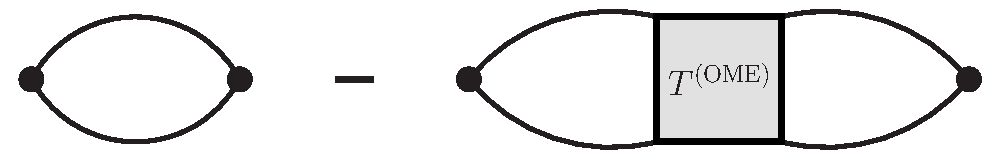
\includegraphics[width=0.62\textwidth]{J.pdf}
\caption{The paper's Fig.~4: $\hat J$ = free two-meson loop between separable vertices minus the same loops with the full OME amplitude inserted.}
\label{fig:J}
\end{figure}

\begin{derbox}[Check in the simplest case \tagD]
Without OME, $T=f\,\tau\,f^T$. Insert into $T=V-VGT$ with $V=fvf^T$: $f\tau f^T=fvf^T-fvf^TGf\,\tau f^T$, i.e.\ $\tau=v-vJ_0\tau$ with $J_0=f^TGf$. Hence $\tau=(1+vJ_0)^{-1}v=(v^{-1}+J_0)^{-1}$. With OME the free loop is replaced by the OME-dressed one, which is the second term of $\hat J$. The same construction for one bare state and a direct meson force is Eq.~(10) of Baru \emph{et al.}\ \tagR{Baru 2010, Eqs.~(10)--(14)}. Watch their sign: their denominator is $E-E_0+{\cal G}$ because they define the loop with the opposite sign.
\end{derbox}

\subsection{Poles}

Bound states are solutions of \tagP{Eq.~(93)}
\begin{equation}
\det\big[\hat v^{-1}(E)+\hat J(E)\big]=0,\qquad \hat v^{-1}={\rm diag}\Big(\frac{E-E_1}{g^2},\dots,\frac{E-E_N}{g^2},\frac1C\Big).
\end{equation}
\begin{derbox}[One bare state, no OME, no contact \tagD]
The condition reduces to $\frac{E-E_1}{g^2}+J_{11}(E)=0$, i.e.
\begin{equation}
E=E_1-g^2J_{11}(E),\qquad J_{11}(E)=\int_0^\Lambda\frac{q^2dq}{2\pi^2}\,f_1(q)^2\,\frac{2\mu}{q^2+\kappa^2}>0\quad(E=-\kappa^2/2\mu).
\end{equation}
Coupling to a continuum that lies \emph{above} pushes a sub-threshold level \emph{down}. This is the self-energy, the Kalashnikova pole equation $M-M_0+g(M)=0$ \tagR{Kalashnikova 2005, Eq.~(6)} in another sign convention. The normalisation (Sect.~\ref{sec:prob}) gives ${\cal P}_{\bar bb}=[1+g^2\partial_EJ_{11}]^{-1}$, the same as Kalashnikova's $Z=[1+\partial_Mg(M)]^{-1}$ \tagR{Kalashnikova 2005, Eq.~(8)}.
\end{derbox}

\textbf{Practical point.} $\TOME$, $X^{\rm in/out}$ and $\hat J$ do not depend on $C$ or $V_0$, so they are computed once per $m_b$. The fit then only inverts small matrices \tagP{l.\,1224}. \texttt{HadronDynamics.jl} implements exactly this reduced matrix, with the compact rows optionally multiplied by $g^2$: $(E-E_n-V_0)+g^2J_{nm}$ \tagR{HadronDynamics.jl, \texttt{src/common/MomentumDynamics.jl}, \texttt{compact\_matrix}}.

\subsection{Fixing $V_0$ and $C$}
For each $m_b\in[4.3,5.3]\GeV$, $C$ and $V_0$ minimise $(\Delta M)^2=\frac13\sum_{n=1}^3(M_n-M_n^{\rm exp})^2$, with $M_n$ from Eq.~(93) at $k=i\kappa_n$, $N=4$, $\Lambda=4\GeV$ \tagP{Eqs.~(94)--(96)}. The fitted $C$ barely moves with $m_b$ ($-16.17$ to $-16.56\GeV^{-2}$), while $V_0$ runs from $820$ to $-1105\MeV$. $V_0$ absorbs the change of $2m_b$ and of the kinetic energy \tagP{Table~III}. This $m_b$ dependence, entering through $E_n^{(0)}$ and $R_{1n}$, is the explicit heavy-quark-mass dependence that the $s$-channel term brings in.

%=====================================================================
\section{What the $s$-channel term does to the states}
\label{sec:effects}
%=====================================================================

\subsection{Compact amplitudes and the compact probability}
\label{sec:prob}

At a bound state $E=-E_B$, Eq.~(55) gives the compact amplitudes \tagP{Eq.~(F12)}
\begin{equation}
\lambda_n=-\frac{g}{E_B+E_n}\int_0^\Lambda\frac{q^2dq}{2\pi^2}f_n^*(q)\Psi_S(q),\qquad
\Pbb=\sum_{n=1}^N|\lambda_n|^2=-\braket{\Psi_S|\partial_EV_S^{(\bar bb)}(E)|\Psi_S}\Big|_{E=-E_B}
\label{eq:Pbb}
\end{equation}
\tagP{Eqs.~(105),(F13)}.
\begin{derbox}[Why the energy derivative \tagD]
$\partial_E\frac{g^2f_nf_n^*}{E-E_n}=-\frac{g^2f_nf_n^*}{(E-E_n)^2}$. Sandwiching between $\Psi_S$ and comparing with $|\lambda_n|^2$ from Eq.~\eqref{eq:Pbb} gives the identity term by term. It is general: if components are eliminated, their norm reappears as $-\braket{\psi|\partial_EV_{\rm eff}|\psi}$ of the effective potential they leave behind. Explicit derivations for bare states: \tagR{Sekihara, Hyodo, Jido 2015, Eqs.~(20),(27),(28); multiple bare states Eq.~(58)} and the generalised sum rule $1=-\sum_{ij}g_ig_j[\delta_{ij}\partial G_i/\partial W+G_i(\partial V_{ij}/\partial W)G_j]$, which ``holds for bound states and resonances, as well as energy dependent or energy independent interactions'' \tagR{Garcia-Recio 2015, Sect.~III Eq.~(9), App.~B}.
The same statement as an operator identity, $\braket{\Psi|\Psi}=\braket{\Psi_M|(1-\partial_E\hat V)|\Psi_M}$, is derived in Sect.~\ref{sec:operator}.
\end{derbox}

The paper's bookkeeping \tagP{Eqs.~(104),(F1)--(F8)}: expand $\hat\tau$ near the pole, $\hat\tau=\bm c\bm c^T/(E+E_B)+\dots$. The couplings satisfy $\bm c^T[\partial_E(\hat v^{-1}+\hat J)]\bm c=1$, which splits into
\begin{equation}
\underbrace{\bm c^T[\partial_E\hat v^{-1}]\bm c=\sum_{n\le N}\frac{c_n^2}{g^2}}_{\Pbb\ (\lambda_n=c_n/g)}\;+\;\underbrace{\bm c^T[\partial_E\hat J]\bm c}_{\sum_\alpha{\cal P}_\alpha+{\cal P}_{3\text{-body}}}=1 .
\end{equation}
\begin{itemize}
\item \textbf{$C$ drops out} of $\Pbb$ because it is energy independent: $\partial_EC=0$ removes the $(N+1)$-th term \tagP{l.\,2358}.
\item The same mechanism, applied to the energy-dependent TOPT OME kernel, gives the three-body probability ${\cal P}_{3\text{-body}}=-\sum\braket{\Psi_{\alpha'}|\partial_EV^{\rm OME}_{\alpha'\alpha}|\Psi_\alpha}$ \tagP{Eq.~(F20)}. A useful unifying sentence for the talk: \emph{the energy dependence of an effective interaction measures the components that were eliminated to produce it} --- compact $\bar bb$ for the $s$-channel term, $B^{(*)}\bar B^{(*)}\phi$ for OME.
\item Caveat: $\Pbb$ is a model-space quantity, well defined for bound states, not a basis-independent observable \tagR{Hyodo 2013, Sect.~3 and summary}. For resonances such quantities become complex \tagR{Cincioglu 2016, Sect.~IV.2}.
\end{itemize}

\subsection{The results of the paper}

\begin{center}
\small
\begin{tabular}{lcccccc}
\toprule
state & mass [GeV] & $E_B$ [MeV] & $\Pbb$ & ${\cal P}_S$ & ${\cal P}_D$ & ${\cal P}_{3\text{-body}}$\\
\midrule
$\chi_{b1}(1P)$ & 9.893 & 711 & 100\% & 0 & 0 & 0\\
$\chi_{b1}(2P)$ & 10.255 & 349 & 98\% & 1\% & 0 & 0\\
$X_b$ (= RPP $\chi_{b1}(3P)$, 10.513) & 10.513 & 91 & 2\% & 41\% & 36\% & 21\%\\
compact $\chi_{b1}(3P)$ (predicted) & 10.544 & 61 & 85\% & 14\% & 1\% & 0\\
\bottomrule
\end{tabular}\\[2pt]
{\footnotesize Central $m_b$, $N=4$, $\Lambda=4\GeV$ \tagP{Table~V}. Over $m_b\in[4.3,5.3]\GeV$ the compact $\chi_{b1}(3P)$ moves from $10.549$ to $10.529\GeV$ and $\Pbb$ from 83\% to 90\%; $X_b$ is pinned by the fit.}
\end{center}

The $s$-channel term is what makes the first two states ``ordinary'' bottomonia ($\Pbb\approx1$) and what produces the second near-threshold pole, the compact $\chi_{b1}(3P)$. The $X_b$ is generated by the hadronic interaction (OME + $C$) and carries only 2\% compact admixture \tagP{l.\,1446}.

\subsection{Avoided level crossing}

\begin{figure}[t]
\centering
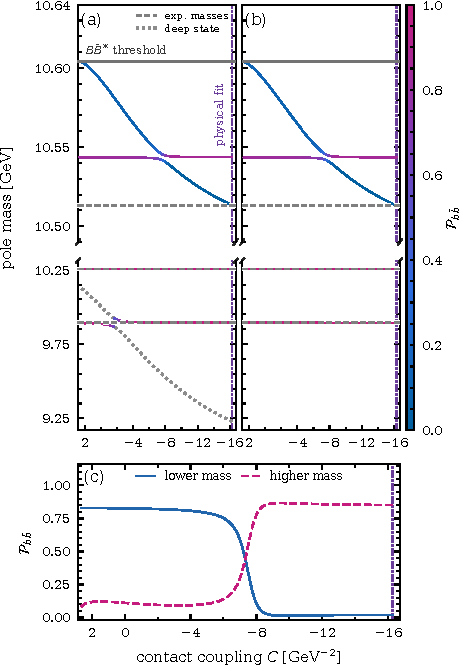
\includegraphics[width=0.48\textwidth]{levels_three_channel_projected.pdf}
\caption{The paper's Fig.~5: pole masses vs the contact coupling $C$ (all else fixed), coloured by $\Pbb$; panel (c) shows $\Pbb$ of the two near-threshold states.}
\label{fig:avoided}
\end{figure}

Vary $C$ with everything else fixed (Fig.~\ref{fig:avoided}). At $C=2.64\GeV^{-2}$ the upper near-threshold state is a $0.1\MeV$-bound, hadron-dominated state and the lower one is compact. As $C$ decreases the two approach, reach a minimum separation of $4\MeV$ at $C=-7.65\GeV^{-2}$, and exchange their compact content. At the fitted $C=-16.27\GeV^{-2}$ the molecular level sits at the experimental $10.513\GeV$ \tagP{l.\,1502--1503}. This is the clearest visualisation of the $s$-channel mixing between the compact $3P$ level and the molecular level.

\textbf{Two-level reading} \tagD{} (approximate): treating the crossing as a two-level problem, the minimum splitting $2|W|=4\MeV$ gives an effective molecule--compact mixing $|W|\approx2\MeV$. At the physical point the two levels are $30\MeV$ apart, so the second-order shift is $\sim W^2/30\MeV\approx0.1\MeV$. This is consistent with the compact state being almost unaffected by the presence of the $X_b$ (next subsection).

\subsection{Diagnostic: switch off OME and $C$}
\label{sec:diag}

\begin{numbox}[$s$-channel exchange alone \tagN]
Take the final model ($g=57.15\MeV$, $V_0=371.5\MeV$, $m_b=4.534\GeV$, $N=4$, $\Lambda=4\GeV$) and set $\VOME=0$ and $C=0$: free $S$-wave $\BBst$ plus the $s$-channel tower only. Solve $\det[(E-E_n)/g^2\,\delta_{nm}+J_{nm}(E)]=0$ with the free loop (\texttt{code/toy.py}):
\begin{center}
\small
\begin{tabular}{lcccc}
\toprule
& bare $E_n$ [MeV] & $s$-channel only [MeV] (${\cal P}_{\bar bb}$) & full LO, paper [MeV] (${\cal P}_{\bar bb}$) & exp.\ $E_B$\\
\midrule
$n=1$ & $-709.6$ & $-713.6$ (99.5\%) & $-711$ (100\%) & 711\\
$n=2$ & $-343.1$ & $-349.4$ (98.7\%) & $-349$ (98\%) & 349\\
$n=3$ & $-42.8$ & $-60.6$ (85.5\%) & $-61$ (85\%), $10.544\GeV$ & ---\\
$X_b$ & --- & none & $-91$ (2\%) & 91\\
\bottomrule
\end{tabular}
\end{center}
The compact sector of the final result, \emph{including the predicted $\chi_{b1}(3P)$ at 10.544 GeV and its 85\% compact content}, is reproduced to $\sim2\MeV$ (1P) and $0.1\MeV$ (3P) by the $s$-channel exchange alone. The bare $3P$ level is pushed down by $18\MeV$ through its coupling to the continuum above it. Of its compact part, $85.25\%$ is $n=3$ and $0.1\%$ each $n=2,4$. Dependence on $N$: the $3P$ level is $-60.26$, $-60.55$, $-60.59$, $-60.60\MeV$ for $N=3,4,5,7$. Without OME and $C$ there is \textbf{no fourth (molecular) state}: the $X_b$ needs the hadronic interaction. The comparison with the full LO numbers indicates that, at the fitted parameters, OME + $C$ barely affect the compact levels.
\end{numbox}

\begin{figure}[t]
\centering
\includegraphics[width=0.95\textwidth]{levels.pdf}
\caption{\tagN{} Level bookkeeping. Reference energies $E_n^{(0)}$ ($V_0=0$), bare energies after the full-fit shift $V_0=371.5\MeV$, $s$-channel-only dressed levels (this note), full LO result (paper, Table V; red: $X_b$), and experiment. Right: zoom near threshold.}
\label{fig:levels}
\end{figure}

\subsection{Diagnostic: what if the coupling were larger?}

\begin{figure}[t]
\centering
\includegraphics[width=0.62\textwidth]{toy_vs_g.pdf}
\caption{\tagN{} Bound states of the $s$-channel-only model ($N=4$, $V_0=371.5\MeV$) versus $g$, coloured by ${\cal P}_{\bar bb}$. A fourth, predominantly hadronic state appears at threshold for $g\approx170\MeV$, three times the lattice-based value.}
\label{fig:toyg}
\end{figure}

\begin{numbox}[Coupling scan \tagN]
In the same $s$-channel-only model, increasing $g$ pushes all levels down. At $g\approx170\MeV$ a fourth state emerges from the threshold, with small compact content: $E=-0.14\MeV$ and ${\cal P}_{\bar bb}=5\%$ at $g=170\MeV$; $-7.1\MeV$, 27\% at $g=200\MeV$; $-32\MeV$, 43\% at $g=250\MeV$. Its compact part is shared between $n=3$ (below) and $n=4$ (above). At the lattice-based $g=57\MeV$ this mechanism is not active. The project's early exploratory fits (older form factors and normalisations) likewise needed couplings well above the lattice value, $g\sim0.15$--$0.4\GeV$, for a molecular pole without OME (\texttt{old/complete-log.tex}, section ``Quark model states only'' and later updates).
\end{numbox}

This is the ``collective state'' mechanism of the papers \BOchiEFT\ builds on \tagP{l.\,243}:
\begin{itemize}
\item In a tower coupled to one channel, ``as soon as the selfenergies get of the order of the level spacing, the pole trajectories bend and the widths decrease again''. ``Which state demonstrates this collective phenomenon \dots depends on the renormalization condition imposed and on the details of the model'' \tagR{Hammer 2016, Sect.~2}.
\item In the strong-coupling limit one pole approaches the zero of the renormalised loop, $k=i\kappa$, which is a bound molecule for $\kappa>0$ and a virtual state for $\kappa<0$. Its residue tends to the Weinberg value, while the other poles decouple with residues $\propto1/g^2$: the molecule does \emph{not} keep a large compact admixture \tagR{Hanhart--Nefediev 2022, Eqs.~(21),(31)--(33),(49)--(51)}. They also warn that ``in more realistic settings, where also $t$- and $u$-channel exchanges are present, this coherence can get spoiled'' \tagR{Hanhart--Nefediev 2022, Sect.~VII}.
\item In \BOchiEFT\ at the lattice coupling, the $X_b$ is not this collective state. It is produced by OME + $C$, and the $s$-channel term supplies the compact partner and the mixing.
\end{itemize}

\subsection{Why the fit improves}
With only quark--antiquark states, $\Delta M_{\rm min}=21\MeV$; in the full LO calculation $\Delta M=0.0$--$4.9\MeV$ over the $m_b$ range \tagP{Table~III}. ``The appearance of the $X_b$ pole between the dressed $\chi_{b1}(2P)$ and $\chi_{b1}(3P)$ states, together with its identification with the experimentally observed state at 10.513 GeV, provides an additional degree of freedom in the fit'' \tagP{l.\,1499}. Be precise in the talk: the improvement is partly a reinterpretation of the third state. If instead $C$ is tuned so that $X_b$ is bound by only $1\MeV$, then $\Delta M=15\MeV$ \tagP{Table~VIII}.

%=====================================================================
\section{Literature map}
\label{sec:lit}
%=====================================================================

\begin{center}
\small
\begin{tabular}{>{\raggedright\arraybackslash}p{3.5cm}>{\raggedright\arraybackslash}p{11.6cm}}
\toprule
Reference & What it contributes (verified) \\
\midrule
Eichten \emph{et al.}\ 1978 & Coupled-channel Cornell model: one interaction for binding and pair creation, below and above threshold (abstract).\\
T\"ornqvist 1985 & Review: meson loops shift masses by up to hundreds of MeV and create multi-quark components (abstract).\\
Kalashnikova 2005 & Block Hamiltonian bare $c\bar c$ + meson pairs, $^3P_0$ vertices; $Z=[1+\partial_Mg]^{-1}$ (Eq.~(8)); option of a near-threshold $D\bar D^*$ virtual state from a bare $2^3P_1$ with tiny $c\bar c$ admixture.\\
Baru \emph{et al.}\ 2010 & One bare state + continuum with direct meson force; $V_{\rm eff}=V+ff/(E-E_0)$ (Eq.~(8)); two-potential solution (Eq.~(10)); $Z=\cos^2\theta$ (Eq.~(17)).\\
Hanhart, Kalashnikova, Nefediev 2011 & Multichannel generalisation (Eqs.~(5)--(22)).\\
Guo \emph{et al.}\ 2016 & Several bare poles, open and hidden flavour channels; $V_{\rm eff}$ with explicit-pole elimination (Eq.~(27)).\\
Hammer, Hanhart, Nefediev 2016 & Collective trajectories in a tower; loops need renormalisation; few-state EFTs are fine at a fixed physical setting; a contact term may replace many $s$-channel poles (Sect.~5).\\
Hanhart, Nefediev 2022 & Analytic strong-coupling limit: molecular pole at the zero of the renormalised loop; compact states decouple (Eqs.~(31)--(33),(49)--(51)).\\
Cincioglu \emph{et al.}\ 2016 & $\chi_{b1}(3P)$ $s$-channel exchange added to a contact EFT; $X_b$ binding vs mixing (Table 4); $4P$ neglected; mixing assumed flavour- and radial-independent.\\
Tarr\'us Castell\`a 2022 & BOEFT with heavy-meson thresholds: mixing Lagrangian projecting onto $\Lambda=0$ (Eq.~(7)); $r$-dependent $V_{\rm mix}$ (Eqs.~(67)--(73)); partial-wave vertices as radial overlaps with $j_{l'}$ (Eq.~(16)).\\
Berwein \emph{et al.}\ 2024; Brambilla \emph{et al.}\ 2026 & BOEFT coupled $\Sigma_g^+/\Sigma_g^{+\prime}/\Pi_g$ equations; $V_{\rm mix}(r)$ profile with $g=50\MeV$ (2604.12603 Eq.~(2.9)); BO--partial-wave recoupling (Eqs.~(4.4)--(4.14)).\\
Bruschini 2023 & HQSS breaking in BO; pseudoscalar-pair source decomposition (Eq.~(3.1a)); $G=-g/2$ (Eq.~(3.3a)); recoupling Table 2.\\
Bulava 2019, 2024; Bali 2005; Bicudo 2019 & Lattice string breaking; mixing values; the factor-2 issue (Sect.~\ref{sec:g}).\\
\bottomrule
\end{tabular}
\end{center}

%=====================================================================
\section{Caveats and open points}
\label{sec:caveats}
%=====================================================================

\begin{enumerate}
\item \textbf{Citation slip (l.\,455):} the chirally extrapolated $\sqrt2g_l\approx50\MeV$ and the mass-dependence figure (Fig.~6) are in Bulava 2024, not Bulava 2019.
\item \textbf{Factor 2:} motivated by the Bicudo reanalysis of Bali's data (ratio $\approx1.9$ at $r/a\approx15$, with refitted energies and angle). For Bulava 2024 it is an approximation pending reanalysis, as the paper says.
\item \textbf{$D$-wave couplings} are present at the BO/HQSS level ($1/\sqrt6$, $-1/\sqrt2$); dropping them at LO is a threshold-momentum argument, not a symmetry selection rule.
\item \textbf{$r$-independent $g$:} the lattice fit model assumption. Lattice and BOEFT analyses find strongly $r$-dependent mixing. The ``subleading $Q^2$'' statement (l.\,459) is the paper's power-counting claim; the cited references do not establish it, and an $r$-profile changes vertex normalisations at ${\cal O}(1)$ for some $n$ (the diagnostic of Sect.~\ref{sec:gassump}).
\item \textbf{${\cal O}(Q^0)$ vertex counting} is an adopted choice; resonance EFTs use different coupling scalings.
\item \textbf{Franck--Condon} references justify the spectator picture, not the precise overlap formula.
\item \textbf{$N\ge4$:} the rationale is not documented (Sect.~\ref{sec:counting}).
\item \textbf{Normalisation identity:} the paper calls its residue relation ``a generalisation'' of Gamermann \emph{et al.}\ and Garcia-Recio \emph{et al.}; Garcia-Recio 2015 Eq.~(9) already includes energy-dependent potentials. The novelty is the separable/OME-dressed bookkeeping, not the $\partial_EV$ term.
\item \textbf{Lattice $\sigma$:} the systematic error from Bulava 2024 Eq.~(10) is not quoted in Table I. Irrelevant at LO without uncertainties \tagP{l.\,940}.
\item \textbf{Project PDF:} \texttt{Xb.pdf} in the folder is the 30 Aug build; equation numbers differ from the current source.
\end{enumerate}

%=====================================================================
\section{Questions you will likely get}
\label{sec:faq}
%=====================================================================

\begin{description}[style=nextline,leftmargin=0.6cm,font=\normalfont\bfseries]
\item[Why ``$s$-channel''? The bottomonium is a bound state, not an exchanged particle.]
In $\BBst\to\bbnP\to\BBst$ the full energy flows through the compact state, which sits in the $s$-channel. Eliminating it from the coupled Schr\"odinger equation gives an energy-dependent $\BBst$ potential with poles at the bare energies, Eqs.~(55)--(58). This is the same as integrating out a dimer field in EFT.

\item[Isn't $C$ plus $s$-channel exchange double counting?]
No. $C$ stands for what is not explicit: states with $n>N$, the high-momentum part of loops, distant thresholds. It changes with $N$ and $\Lambda$ (Tables IV, VI), and observables do not. The split between explicit and contact contributions is scheme dependent.

\item[Where does $57\MeV$ come from?]
$\sqrt2g_l=49.5\MeV$ (Bulava 2024, physical point), times 2 (overlap of the pseudoscalar-pair operator with $\Sigma_g^{+\prime}$, Bicudo/Bruschini), times $1/\sqrt3$ (the $S$-wave share of $\Sigma_g^{+\prime}$).

\item[Why is the vertex a $j_0$ transform of a $P$-wave function?]
The $b\bar b$ separation is unchanged (Franck--Condon), and the orbital $L=1$ is transferred into the light spin ($\Sigma_g^{+\prime}$, $j_\ell=1$ along $\hat{\bm r}$). The isotropic part is the $S$-wave pair with the same radial function; the angular algebra is in $g$.

\item[Why only the $S$ wave?]
LO. The $D$-wave couplings exist ($1/\sqrt6$, $-1/\sqrt2$), but their vertices start at ${\cal O}(p^2)$ in the overlap. They enter at higher order and turn $\VQQ$ into a channel matrix.

\item[Why is $V_0$ free if the lattice gives $\hat V_0$?]
The lattice is static. $V_0$ absorbs the $m_b$ choice, spin-dependent corrections ($\lesssim1\MeV$ variation), and static-to-physical differences. In the coupled problem it fixes the bare levels relative to the threshold, which the $s$-channel potential is very sensitive to.

\item[Why truncate at $N$, and why $N=4$?]
States far from the energies of interest give contributions analytic in $E$ and $p$, absorbable into contacts; the near ones must be explicit. $N=4$--7 give the same physics with $C$ changing by $0.01\GeV^{-2}$ (Table IV). The ``$N\ge4$'' condition is stated without documented reason (Sect.~\ref{sec:counting}).

\item[How do you know which pole is the $X_b$?]
By its composition, $\Pbb=2\%$, and by following the trajectories in $C$ (Fig.~5), where the two near-threshold poles exchange their compact content through an avoided crossing.

\item[What fixes the predicted $\chi_{b1}(3P)$ at $10.544\GeV$?]
In the paper: $10.529$--$10.549\GeV$ over $m_b\in[4.3,5.3]$; $E_B=60$--$61\MeV$ for $\Lambda=3$--5 GeV (Table VI); within $\sim3\MeV$ under the OME approximations of Table VII. Diagnostic (this note): the $s$-channel exchange alone reproduces it within $0.1\MeV$. It is set by the bare $3P$ position (via $V_0$, fixed by $1P$/$2P$) plus the continuum self-energy (via $g$ and $f_3$). The D0 peak at $10.551\pm0.014\pm0.017\GeV$ is compatible with it \tagP{l.\,1750}.

\item[Is ${\cal P}_{\bar bb}$ measurable?]
No. It is defined within the model space and well defined for bound states. Its value depends on the basis and scheme.

\item[Could the $s$-channel exchange alone make the $X_b$?]
Not at $g=57\MeV$. In the $s$-channel-only diagnostic a near-threshold molecular state appears only for $g\gtrsim170\MeV$. The collective-state mechanism of Hammer \emph{et al.}\ and Hanhart--Nefediev needs strong coupling.

\item[How is this different from BOEFT?]
BOEFT solves coupled $r$-space equations with $\Sigma_g^+$, $\Sigma_g^{+\prime}$, $\Pi_g$ potentials and an $r$-dependent $V_{\rm mix}(r)$. \BOchiEFT\ puts the mixing into the separable $s$-channel vertex, $g\,\psi_n(p)$, and treats the hadron--hadron force with $\chi$EFT (OME + contacts) in momentum space \tagP{Sect.~IV\,F}. The BOEFT papers use a plateau value $g=50\MeV$ for the full $\Sigma_g^+$--$\Sigma_g^{+\prime}$ mixing \tagR{Brambilla 2026 (2604.12603), Eq.~(2.9)}; by the argument of Sect.~\ref{sec:g} this lacks the factor 2 ($2\sqrt2g_l\approx99\MeV$).
\end{description}

%=====================================================================
\section{Self-check questions}
\label{sec:selfcheck}
%=====================================================================

Work these out on paper before reading the answers in Appendix~\ref{app:answers}.
\begin{enumerate}
\item Derive Eq.~(55) and then Eq.~(57) from Eq.~(49). Which step would fail if the bare states had direct mutual couplings?
\item Show $\int\frac{p^2dp}{2\pi^2}f_nf_m=\delta_{nm}$. What does it imply for $\sum_nf_n(p')f_n(p)$?
\item Why is the $s$-channel term attractive just below a bare level and repulsive just above? Which bare states repel and which attract at threshold?
\item In the single-state limit, show that the bound level lies below the bare one. What happens for a bare state above threshold?
\item Why does $C$ not contribute to $\Pbb$? What would change if $C$ were energy dependent?
\item Using Eq.~(14), find the overlap of $\ket{B\bar B}$ with $\ket{1_\ell,0}\ket{1_{\bar bb},0}$. Why does only this component couple to the string?
\item Reproduce the $1/3$ $S$-wave fraction of $\Sigma_g^{+\prime}$ with the Cartesian argument.
\item Why does $V_0$ matter beyond an overall shift once the continuum is included?
\item If $g$ doubled, which state would move most, and why?
\item Why can the higher states ($n\ge5$) have larger $f_n(0)$ than the lower ones but still be negligible near threshold?
\item What does the two-potential formula buy you numerically in the fit?
\item Where in the paper does the explicit $m_Q$ dependence enter through the $s$-channel term?
\item Redo the derivation of Eq.~(58) with projectors only, without $\lambda_n$ or $\phi(q)$. Where exactly does the $1/(4\pi)$ come from, and why is Eq.~(46) then automatic?
\item Show that $B\bar B$ can never be $1^{++}$, and that $B^*\bar B^*(^3S_1)$ is $1^{+-}$.
\item Why is there no $1^{++}$ channel with $L\ge4$? Why none with odd $L$?
\item Using $\eta=CP$ and $\sigma=P(-1)^{j_\ell}$, derive the labels $\Sigma_g^{+\prime}$, $\Pi_g$ and $\Sigma_u^-$ of the $S$-wave pair configurations. Why does the string mix only with $\Sigma_g^{+\prime}$?
\item Why is there no $\Sigma$ configuration with $J_\ell=2$ in the $1^{++}$ sector?
\item Why is the $S$-wave $1^{++}$ pair pure $s_{\bar bb}=1$, $j_\ell=1$, while the $S$-wave $B\bar B$ pair is not?
\item Why does the pion couple $B^*$ to $B$ in a $P$ wave, and why does that generate a tensor force?
\end{enumerate}

%=====================================================================
\section{A possible storyline for the talk}
%=====================================================================

\begin{enumerate}
\item \emph{The puzzle.} The $1^{++}$ spectrum near the $\BBst$ threshold; the quark model misses the level compression (66 vs 104 MeV); hadronic EFTs need the unknown $m_Q$ scaling of contacts.
\item \emph{What QCD tells us.} Lattice string breaking (Fig.~\ref{fig:lattice}): a string level and a meson-pair level mixing with $g_l$.
\item \emph{From the static picture to hadrons.} BO selection ($\Sigma_g^+\leftrightarrow\Sigma_g^{+\prime}$ only); Franck--Condon (Fig.~\ref{fig:transition}); vertex $g\psi_n(p)$ with $j_0$ (Fig.~\ref{fig:fn}).
\item \emph{The number.} $g=\sqrt2\times2\times\frac1{\sqrt3}\times g_l=57\MeV$.
\item \emph{The potential.} Matrix Hamiltonian $\to$ eliminate the tower $\to$ Eq.~(58); energy dependence (Fig.~\ref{fig:VE}).
\item \emph{EFT logic.} Power counting, truncation $N$, contact $C$ (Tables IV, VI).
\item \emph{Solving it.} Separable form, two-potential LSE, $\det(\hat v^{-1}+\hat J)=0$.
\item \emph{What it does.} Level shifts and $\Pbb$; avoided crossing (Fig.~\ref{fig:avoided}); the compact $\chi_{b1}(3P)$ at $10.544\GeV$; the $X_b$ needs OME + $C$.
\item \emph{Caveats.} The factor 2, constant $g$, $D$-wave couplings at higher order.
\end{enumerate}

\appendix

%=====================================================================
\section{Notation and numbers}
%=====================================================================

\begin{center}
\small
\begin{tabular}{lll}
\toprule
symbol & meaning & value / source\\
\midrule
$\Mth$ & $m_B+m_{B^*}$ & $10.604\GeV$ (code: $10.60427$) \tagP{Eq.~(3)}\\
$\mu$ & $\BBst$ reduced mass & $2.651\GeV$ \tagP{Eq.~(3)}\\
$E$, $k$ & $M-\Mth$, $E=k^2/2\mu$ & \tagP{Eqs.~(4),(5)}\\
$m_b$ & bottom-quark mass in $H$ & $4.534\GeV$ (scan 4.3--5.3) \tagP{Eq.~(39)}\\
$M_n^{(0)}$, $E_n^{(0)}$ & reference masses/energies ($V_0=0$) & \tagP{Table~II}\\
$E_n=E_n^{(0)}+V_0$ & bare energies & $V_0=371\MeV$ (full fit), $353\MeV$ (QM only)\\
$R_{1n}$, $u_n$ & radial function, $u_n=rR_{1n}$ & \tagP{Eqs.~(40),(A1)}\\
$\psi_n(p)$ & $4\pi\int r^2dr\,j_0(pr)R_{1n}(r)$ & \tagP{Eq.~(53)}\\
$f_n(p)$ & $\psi_n/\sqrt{4\pi}$ ($n\le N$), $1$ ($n=N+1$) & \tagP{Eq.~(61)}\\
$g$ & $S$-wave $[\bar bb]_1\BBst$ coupling & $57\MeV$ \tagP{Eq.~(18)}\\
$g_l$ & lattice mixing per light flavour & $35\MeV$ \tagP{Table~I}\\
$v_n$ & $g^2/(E-E_n)$ ($n\le N$), $C$ & \tagP{Eq.~(63)}\\
$C$ & contact term & $-16.27\GeV^{-2}$ ($\Lambda=4\GeV$, $N=4$) \tagP{Table~III}\\
$\lambda_n$, $c_n$ & compact amplitudes, $\lambda_n=c_n/g$ & \tagP{Eqs.~(F11),(F12)}\\
$\Pbb$ & $\sum_n|\lambda_n|^2$ & \tagP{Eq.~(105)}\\
\bottomrule
\end{tabular}
\end{center}

%=====================================================================
\section{Reproduction scripts}
%=====================================================================

The \tagN{} results come from the Python scripts in \texttt{code/} (NumPy/SciPy/Matplotlib; run with \texttt{uv run --no-project --with numpy --with scipy --with matplotlib python <script>} from inside \texttt{code/}):
\begin{itemize}
\item \texttt{cornell.py}: finite-difference $P$-wave Cornell solver on the grid of App.~A ($N_r=12000$, $r_{\rm box}=30\GeV^{-1}$), $j_0$ form factors, and the checks printed in the reproduction box (masses, $V_0^{(\bar bb)}$, level spacings, normalisation, radii);
\item \texttt{toy.py}: the $s$-channel-only pole search and compact probabilities (Sect.~\ref{sec:diag});
\item \texttt{rdep.py}: the $r$-profile diagnostic (Sect.~\ref{sec:gassump});
\item \texttt{qnumbers.py}: the quantum-number checks of Sect.~\ref{sec:qn} (heavy/light spin decompositions, 6$j$ and Clebsch--Gordan recouplings, the BO matrix, projector normalisations, App.~B angular factors); run with \texttt{--with numpy --with sympy};
\item \texttt{figs.py}: all \tagN{} figures; \texttt{python figs.py ../figs}.
\end{itemize}
The script does not integrate the WKB/Numerov tail used in the paper. For real momenta this is irrelevant (the box is $3\times$ the outer turning point of $n=7$), and it reproduces Table II exactly. The scripts were not cross-checked against \texttt{HadronDynamics.jl}: its pinned private dependency (\texttt{ThreeBodyToolkit.jl} at the commit in \texttt{Manifest.toml}) could not be installed offline. A direct cross-check of the $s$-channel-only diagnostic with the real code is the natural next step: set the pion coupling to zero and make the contact negligible.

%=====================================================================
\section{Answers to the self-check questions}
\label{app:answers}
%=====================================================================

\begin{enumerate}
\item Solve Eq.~\eqref{eq:sys1} for $\lambda_n$ and insert into Eq.~\eqref{eq:sys2}. With direct bare--bare couplings the compact block is no longer diagonal; one inverts the matrix $(E-H_{\rm compact})$, and the potential becomes $\hat g(E-H_{\rm compact})^{-1}\hat g$. Diagonalising $H_{\rm compact}$ first brings it back to the same form.
\item Unitarity of the $j_0$ transform plus orthonormality of $R_{1n}$. Completeness gives $\sum_nf_n(p')f_n(p)=\frac{2\pi^2}{p^2}\delta(p-p')$: the tower with \emph{degenerate} energies would be local.
\item Sign of $1/(E-E_n)$. At threshold ($E\approx0$), states below threshold ($n\le3$) repel and states above ($n\ge4$) attract.
\item $J_{11}>0$ below threshold, so $E=E_1-g^2J_{11}<E_1$. A bare state above threshold acquires a width: the loop develops an imaginary part, the pole moves into the complex plane (resonance).
\item $\partial_EC=0$. An energy-dependent contact would contribute $-\braket{\Psi|\partial_EC|\Psi}$, i.e.\ it would represent an eliminated component not included in $\Pbb$.
\item $-1/2$. The string has light degrees of freedom in the vacuum and heavy spin $\ket{1,0}$; HQSS conserves the heavy spin, and BO symmetry restricts the light state to $\Sigma_g^{+\prime}$, i.e.\ $\ket{1_\ell,0}$.
\item See the box in Sect.~\ref{sec:vertex}.
\item The threshold does not move with $V_0$. $V_0$ sets $E_n$ relative to the continuum and therefore the size and sign of each $1/(E-E_n)$.
\item The compact $3P$ (closest to threshold, enhanced propagator). In the diagnostic, $g=100\MeV$ moves it from $-61$ to $-87\MeV$, but $1P$ only from $-714$ to $-722\MeV$.
\item Their energy denominators are large ($E_n\gtrsim460\MeV$ above threshold), so near threshold their contribution is small and nearly energy independent, i.e.\ close to a constant that $C$ absorbs. In the diagnostic their total compact admixture in the $3P$ state is $\lesssim0.01\%$.
\item $\TOME$, $X$ and $\hat J$ are independent of $C$ and $V_0$, so each fit step is a small matrix inversion.
\item Through $E_n^{(0)}$ and $R_{1n}$, both computed from $H$ with the chosen $m_b$ (Table III, Table V).
\item See Sect.~\ref{sec:operator}. The $1/(4\pi)$ is $(\sqrt{4\pi}/4\pi)^2$: each overlap $\braket{p,S|\tilde n}$ produces $\int d\Omega\,Y_{00}=\sqrt{4\pi}$, while $\psi_n$ was defined with $4\pi$. Eq.~(46) follows from $\braket{\Psi|(P_Q+P_M)|\Psi}=\braket{\Psi_M|(1-\partial_E\hat V)|\Psi_M}$.
\item $B\bar B$ has $S=0$, so $J=L$, $P=(-1)^L$, $C=(-1)^L$: $J=1$ forces $1^{--}$. $B^*\bar B^*$ with $S=1$, $L=0$: $P=+$, $C=(-1)^{0+1}=-$, so $1^{+-}$.
\item $L\ge4$ with $S\le2$ gives $J\ge L-S\ge2$. Odd $L$ gives $P=(-1)^L=-$.
\item $1^{--}$: $\eta=(-)(-)=g$; $\lambda_\ell=0$ gives $\sigma=(-1)(-1)^1=+$, hence $\Sigma_g^+$ (primed), and $|\lambda_\ell|=1$ gives $\Pi_g$. $0^{-+}$: $\eta=(-)(+)=u$, $\sigma=(-1)(-1)^0=-$, hence $\Sigma_u^-$. In the static limit only states with identical BO labels mix; the string is $\Sigma_g^+$.
\item $\braket{L\,0\,1\,0|J_\ell\,0}=0$ for $J_\ell=L$, and $J_\ell=2$ only arises from $L=2$.
\item By the $PC$ rule, $1^{++}$ arises only from $1_\ell^{--}\otimes1_{\bar bb}^{--}$. $0^{++}$ arises from both $0\otimes0$ and $(1\otimes1)_0$, so $B\bar B$ is a mixture ($\frac12$, $\frac{\sqrt3}{2}$).
\item $0^-\to0^-0^-$ is forbidden by parity, while $1^-\to0^-0^-$ needs $L=1$. Each vertex is then linear in $\bm q$; the product $q_iq_j$ contains a rank-2 piece that changes $L$ by 2.
\end{enumerate}

%=====================================================================
\begin{thebibliography}{99}
\small
\bibitem{Xb} Y.~Zhang, F.-K.~Guo, C.~Hanhart, A.~Nefediev, P.~P\"utz, \emph{Born--Oppenheimer chiral effective field theory and its application to $X_b$} (this project, \texttt{Xb.tex}).
\bibitem{Bulava2024} J.~Bulava \emph{et al.}, PLB 854 (2024) 138754, arXiv:2403.00754.
\bibitem{Bulava2019} J.~Bulava \emph{et al.}, PLB 793 (2019) 493, arXiv:1902.04006.
\bibitem{Bali2005} G.~S.~Bali \emph{et al.}, PRD 71 (2005) 114513, hep-lat/0505012.
\bibitem{Bicudo2019} P.~Bicudo, M.~Cardoso, N.~Cardoso, M.~Wagner, PRD 101 (2020) 034503, arXiv:1910.04827.
\bibitem{Bruschini2023} R.~Bruschini, JHEP 08 (2023) 219, arXiv:2303.17533.
\bibitem{Bondar2011} A.~E.~Bondar \emph{et al.}, PRD 84 (2011) 054010, arXiv:1105.4473.
\bibitem{Baru2016} V.~Baru \emph{et al.}, PLB 763 (2016) 20, arXiv:1605.09649.
\bibitem{Tarrus2022} J.~Tarr\'us Castell\`a, PRD 106 (2022) 094020, arXiv:2207.09365.
\bibitem{Berwein2024} M.~Berwein \emph{et al.}, PRD 110 (2024) 094040, arXiv:2408.04719.
\bibitem{Brambilla2026} N.~Brambilla \emph{et al.}, \emph{Open-flavor threshold effects on quarkonium spectrum in the BOEFT}, arXiv:2604.12603.
\bibitem{Eichten1978} E.~Eichten \emph{et al.}, PRD 17 (1978) 3090.
\bibitem{Tornqvist1985} N.~A.~T\"ornqvist, Acta Phys.\ Polon.\ B16 (1985) 503.
\bibitem{Kalashnikova2005} Yu.~S.~Kalashnikova, PRD 72 (2005) 034010, hep-ph/0506270.
\bibitem{Baru2010} V.~Baru \emph{et al.}, EPJA 44 (2010) 93, arXiv:1001.0369.
\bibitem{Hanhart2011} C.~Hanhart, Yu.~S.~Kalashnikova, A.~V.~Nefediev, EPJA 47 (2011) 101, arXiv:1106.1185.
\bibitem{Guo2016} F.-K.~Guo \emph{et al.}, PRD 93 (2016) 074031, arXiv:1602.00940.
\bibitem{Hammer2016} I.~K.~Hammer, C.~Hanhart, A.~V.~Nefediev, EPJA 52 (2016) 330, arXiv:1607.06971.
\bibitem{Hanhart2022} C.~Hanhart, A.~Nefediev, PRD 106 (2022) 114003, arXiv:2209.10165.
\bibitem{Cincioglu2016} E.~Cincioglu \emph{et al.}, EPJC 76 (2016) 576, arXiv:1606.03239.
\bibitem{Bedaque2003} P.~F.~Bedaque, H.-W.~Hammer, U.~van Kolck, PLB 569 (2003) 159, nucl-th/0304007.
\bibitem{Alhakami2017} M.~H.~Alhakami, PRD 96 (2017) 056019, arXiv:1706.05622.
\bibitem{Habashi2021} J.~B.~Habashi, S.~Fleming, U.~van Kolck, EPJA 57 (2021) 169, arXiv:2012.14995; and J.~B.~Habashi \emph{et al.}, Annals Phys.\ 422 (2020) 168283, arXiv:2007.07360.
\bibitem{Guo2011} F.-K.~Guo \emph{et al.}, PRD 83 (2011) 034013, arXiv:1008.3632.
\bibitem{LlanesEstrada2008} F.~J.~Llanes-Estrada \emph{et al.}, AIP Conf.\ Proc.\ 1030 (2008) 171, arXiv:0803.0806.
\bibitem{TorresRincon2010} J.~M.~Torres-Rincon, F.~J.~Llanes-Estrada, PRL 105 (2010) 022003, arXiv:1003.5989.
\bibitem{Gamermann2010} D.~Gamermann \emph{et al.}, PRD 81 (2010) 014029, arXiv:0911.4407.
\bibitem{GarciaRecio2015} C.~Garcia-Recio \emph{et al.}, PRD 92 (2015) 034011, arXiv:1506.04235.
\bibitem{Hyodo2013} T.~Hyodo, IJMPA 28 (2013) 1330045, arXiv:1310.1176.
\bibitem{Sekihara2015} T.~Sekihara, T.~Hyodo, D.~Jido, PTEP 2015 063D04, arXiv:1411.2308.
\bibitem{HD} \texttt{HadronDynamics.jl} (fkguo/HadronDynamics.jl, commit \texttt{91ee258}), \texttt{docs/BOCHIEFT.md}, \texttt{docs/BOCHIEFT\_TUTORIAL.md}, \texttt{data/bochiEFT/central.toml}.
\end{thebibliography}

\end{document}
